\pdfoutput=1
%% Author: PGL  Porta Mana
%% Created: 2015-05-01T20:53:34+0200
%% Last-Updated: 2018-04-08T02:08:37+0200
%%%%%%%%%%%%%%%%%%%%%%%%%%%%%%%%%%%%%%%%%%%%%%%%%%%%%%%%%%%%%%%%%%%%%%
% Report-no: ***
\newif\ifarxiv
\arxivfalse
\ifarxiv\pdfmapfile{+classico.map}\fi
\newif\ifafour
\afourfalse % true = A4, false = A5
\newif\iftypodisclaim % typographical disclaim on the side
\typodisclaimtrue
\newif\ifpublic
\publictrue % true = for publication, false = personal notes
\newcommand*{\memfontfamily}{zplx}
\newcommand*{\memfontpack}{newpxtext}
\documentclass[\ifafour a4paper,12pt,\else a5paper,10pt,\fi%extrafontsizes,%
onecolumn,oneside,article,%french,italian,german,swedish,latin,
british%
]{memoir}
\newif\ifpublic
\publictrue % true = for publication, false = personal notes
\newcommand*{\firstdraft}{16 October 2016}
\newcommand*{\firstpublished}{20 February 2018}
\newcommand*{\oggi}{\today}
\newcommand*{\propertitle}{Force, inertia, metric\\ in Newtonian relativity and general relativity}
\newcommand*{\pdftitle}{Force, inertia, metric in Newtonian and general relativity}
\newcommand*{\headtitle}{Force, inertia, metric in Newtonian and general relativity}
\newcommand*{\pdfauthor}{P.G.L.  Porta Mana}
\newcommand*{\headauthor}{\ifpublic\autanet\ Porta Mana%
\else\autanet\ Luca\fi}
\newcommand*{\reporthead}{}
%%%%%%%%%%%%%%%%%%%%%%%%%%%%%%%%%%%%%%%%%%%%%%%%%%%%%%%%%%%%%%%%%%%%%%%%%%%%
%%%%%%%%%%%%%%%%%%%%%%%%%%%%%%%%%%%%%%%%%%%%%%%%%%%%%%%%%%%%%%%%%%%%%%%%%%%%
%\usepackage{pifont}
%\usepackage{fontawesome}
\usepackage[T1]{fontenc} 
\input{glyphtounicode} \pdfgentounicode=1
\usepackage[utf8]{inputenx}
%\usepackage{newunicodechar}
% \newunicodechar{Ĕ}{\u{E}}
% \newunicodechar{ĕ}{\u{e}}
% \newunicodechar{Ĭ}{\u{I}}
% \newunicodechar{ĭ}{\u{\i}}
% \newunicodechar{Ŏ}{\u{O}}
% \newunicodechar{ŏ}{\u{o}}
% \newunicodechar{Ŭ}{\u{U}}
% \newunicodechar{ŭ}{\u{u}}
% \newunicodechar{Ā}{\=A}
% \newunicodechar{ā}{\=a}
% \newunicodechar{Ē}{\=E}
% \newunicodechar{ē}{\=e}
% \newunicodechar{Ī}{\=I}
% \newunicodechar{ī}{\={\i}}
% \newunicodechar{Ō}{\=O}
% \newunicodechar{ō}{\=o}
% \newunicodechar{Ū}{\=U}
% \newunicodechar{ū}{\=u}
% \newunicodechar{Ȳ}{\=Y}
% \newunicodechar{ȳ}{\=y}

\newcommand*{\bmmax}{0} % reduce number of bold fonts, before bm
\newcommand*{\hmmax}{0} % reduce number of heavy fonts, before bm
\usepackage{textcomp}
\usepackage[normalem]{ulem}
% \makeatletter
% \def\ssout{\bgroup \ULdepth=-.35ex%\UL@setULdepth
%  \markoverwith{\lower\ULdepth\hbox
%    {\kern-.03em\vbox{\hrule width.2em\kern1.2\p@\hrule}\kern-.03em}}%
%  \ULon}
% \makeatother
\usepackage{amsmath}
\usepackage{mathtools}
\usepackage{empheq}% automatically calls amsmath and mathtools
\newcommand*{\widefbox}[1]{\fbox{\hspace{1em}#1\hspace{1em}}}
\setlength{\multlinegap}{0pt}
%\usepackage{fancybox}
\usepackage{framed}
% \usepackage[misc]{ifsym} % for dice
% \newcommand*{\diceone}{{\scriptsize\Cube{1}}}
\usepackage{amssymb}
\usepackage{amsxtra}

\usepackage[main=british,french,italian,german,swedish,latin,esperanto]{babel}\selectlanguage{british}
\newcommand*{\langfrench}{\foreignlanguage{french}}
\newcommand*{\langgerman}{\foreignlanguage{german}}
\newcommand*{\langitalian}{\foreignlanguage{italian}}
\newcommand*{\langswedish}{\foreignlanguage{swedish}}
\newcommand*{\langlatin}{\foreignlanguage{latin}}
\newcommand*{\langnohyph}{\foreignlanguage{nohyphenation}}

\usepackage[autostyle=false,autopunct=false,english=british]{csquotes}
\setquotestyle{british}

\usepackage{amsthm}
\newcommand*{\QED}{\textsc{q.e.d.}}
\renewcommand*{\qedsymbol}{\QED}
\theoremstyle{remark}
\newtheorem{note}{Note}
\newtheorem*{remark}{Note}
\newtheoremstyle{innote}{\parsep}{\parsep}{\footnotesize}{}{}{}{0pt}{}
\theoremstyle{innote}
\newtheorem*{innote}{}


\usepackage[shortlabels,inline]{enumitem}
\SetEnumitemKey{para}{itemindent=\parindent,leftmargin=0pt,listparindent=\parindent,parsep=0pt,itemsep=\topsep}
% \begin{asparaenum} = \begin{enumerate}[para]
% \begin{inparaenum} = \begin{enumerate*}
\setlist[enumerate,2]{label=\alph*.}
\setlist[enumerate]{leftmargin=\parindent}
\setlist[itemize]{leftmargin=\parindent}
\setlist[description]{leftmargin=\parindent}

\usepackage[babel,theoremfont]{newpxtext}
\usepackage[bigdelims,nosymbolsc%,smallerops % probably arXiv doesn't have it
]{newpxmath}
\useosf\linespread{1.083}
%% smaller operators for old version of newpxmath
\makeatletter
\def\re@DeclareMathSymbol#1#2#3#4{%
    \let#1=\undefined
    \DeclareMathSymbol{#1}{#2}{#3}{#4}}
%\re@DeclareMathSymbol{\bigsqcupop}{\mathop}{largesymbols}{"46}
%\re@DeclareMathSymbol{\bigodotop}{\mathop}{largesymbols}{"4A}
\re@DeclareMathSymbol{\bigoplusop}{\mathop}{largesymbols}{"4C}
\re@DeclareMathSymbol{\bigotimesop}{\mathop}{largesymbols}{"4E}
\re@DeclareMathSymbol{\sumop}{\mathop}{largesymbols}{"50}
\re@DeclareMathSymbol{\prodop}{\mathop}{largesymbols}{"51}
\re@DeclareMathSymbol{\bigcupop}{\mathop}{largesymbols}{"53}
\re@DeclareMathSymbol{\bigcapop}{\mathop}{largesymbols}{"54}
%\re@DeclareMathSymbol{\biguplusop}{\mathop}{largesymbols}{"55}
\re@DeclareMathSymbol{\bigwedgeop}{\mathop}{largesymbols}{"56}
\re@DeclareMathSymbol{\bigveeop}{\mathop}{largesymbols}{"57}
%\re@DeclareMathSymbol{\bigcupdotop}{\mathop}{largesymbols}{"DF}
%\re@DeclareMathSymbol{\bigcapplusop}{\mathop}{largesymbolsPXA}{"00}
%\re@DeclareMathSymbol{\bigsqcupplusop}{\mathop}{largesymbolsPXA}{"02}
%\re@DeclareMathSymbol{\bigsqcapplusop}{\mathop}{largesymbolsPXA}{"04}
%\re@DeclareMathSymbol{\bigsqcapop}{\mathop}{largesymbolsPXA}{"06}
\re@DeclareMathSymbol{\bigtimesop}{\mathop}{largesymbolsPXA}{"10}
%\re@DeclareMathSymbol{\coprodop}{\mathop}{largesymbols}{"60}
%\re@DeclareMathSymbol{\varprod}{\mathop}{largesymbolsPXA}{16}
\makeatother


%% With euler font cursive for Greek letters - the [1] means 100% scaling
\DeclareFontFamily{U}{egreek}{\skewchar\font'177}%
\DeclareFontShape{U}{egreek}{m}{n}{<-6>s*[1]eurm5 <6-8>s*[1]eurm7 <8->s*[1]eurm10}{}%
\DeclareFontShape{U}{egreek}{m}{it}{<->s*[1]eurmo10}{}%
\DeclareFontShape{U}{egreek}{b}{n}{<-6>s*[1]eurb5 <6-8>s*[1]eurb7 <8->s*[1]eurb10}{}%
\DeclareFontShape{U}{egreek}{b}{it}{<->s*[1]eurbo10}{}%
\DeclareSymbolFont{egreeki}{U}{egreek}{m}{it}%
\SetSymbolFont{egreeki}{bold}{U}{egreek}{b}{it}% from the amsfonts package
\DeclareSymbolFont{egreekr}{U}{egreek}{m}{n}%
\SetSymbolFont{egreekr}{bold}{U}{egreek}{b}{n}% from the amsfonts package
% Take also \sum, \prod, \coprod symbols from Euler fonts
\DeclareFontFamily{U}{egreekx}{\skewchar\font'177}
\DeclareFontShape{U}{egreekx}{m}{n}{%
       <-7.5>s*[0.9]euex7%
    <7.5-8.5>s*[0.9]euex8%
    <8.5-9.5>s*[0.9]euex9%
    <9.5->s*[0.9]euex10%
}{}
\DeclareSymbolFont{egreekx}{U}{egreekx}{m}{n}
\DeclareMathSymbol{\sumop}{\mathop}{egreekx}{"50}
\DeclareMathSymbol{\prodop}{\mathop}{egreekx}{"51}
\DeclareMathSymbol{\coprodop}{\mathop}{egreekx}{"60}
\makeatletter
\def\sum{\DOTSI\sumop\slimits@}
\def\prod{\DOTSI\prodop\slimits@}
\def\coprod{\DOTSI\coprodop\slimits@}
\makeatother
\ifarxiv\else\input{undefinegreek.tex}\fi% make sure no CMF greek letters sneak in
% Greek letters not usually given in LaTeX. Comment the unneeded ones
% \DeclareMathSymbol{\varpartial}{\mathalpha}{egreeki}{"40}
 \DeclareMathSymbol{\partialup}{\mathalpha}{egreekr}{"40}
 \DeclareMathSymbol{\alpha}{\mathalpha}{egreeki}{"0B}
 \DeclareMathSymbol{\beta}{\mathalpha}{egreeki}{"0C}
 \DeclareMathSymbol{\gamma}{\mathalpha}{egreeki}{"0D}
% \DeclareMathSymbol{\delta}{\mathalpha}{egreeki}{"0E}
 \DeclareMathSymbol{\epsilon}{\mathalpha}{egreeki}{"0F}
% \DeclareMathSymbol{\zeta}{\mathalpha}{egreeki}{"10}
 \DeclareMathSymbol{\eta}{\mathalpha}{egreeki}{"11}
 \DeclareMathSymbol{\theta}{\mathalpha}{egreeki}{"12}
% \DeclareMathSymbol{\iota}{\mathalpha}{egreeki}{"13}
 \DeclareMathSymbol{\kappa}{\mathalpha}{egreeki}{"14}
 \DeclareMathSymbol{\lambda}{\mathalpha}{egreeki}{"15}
% \DeclareMathSymbol{\mu}{\mathalpha}{egreeki}{"16}
 \DeclareMathSymbol{\nu}{\mathalpha}{egreeki}{"17}
% \DeclareMathSymbol{\xi}{\mathalpha}{egreeki}{"18}
% \DeclareMathSymbol{\omicron}{\mathalpha}{egreeki}{"6F}
% \DeclareMathSymbol{\pi}{\mathalpha}{egreeki}{"19}
 \DeclareMathSymbol{\rho}{\mathalpha}{egreeki}{"1A}
% \DeclareMathSymbol{\sigma}{\mathalpha}{egreeki}{"1B}
 \DeclareMathSymbol{\tau}{\mathalpha}{egreeki}{"1C}
% \DeclareMathSymbol{\upsilon}{\mathalpha}{egreeki}{"1D}
% \DeclareMathSymbol{\phi}{\mathalpha}{egreeki}{"1E}
% \DeclareMathSymbol{\chi}{\mathalpha}{egreeki}{"1F}
% \DeclareMathSymbol{\psi}{\mathalpha}{egreeki}{"20}
% \DeclareMathSymbol{\omega}{\mathalpha}{egreeki}{"21}
% \DeclareMathSymbol{\varepsilon}{\mathalpha}{egreeki}{"22}
% \DeclareMathSymbol{\vartheta}{\mathalpha}{egreeki}{"23}
% \DeclareMathSymbol{\varpi}{\mathalpha}{egreeki}{"24}
% \let\varrho\rho 
% \let\varsigma\sigma
 \let\varkappa\kappa
% \DeclareMathSymbol{\varphi}{\mathalpha}{egreeki}{"27}
% %
% \DeclareMathSymbol{\varAlpha}{\mathalpha}{egreeki}{"41}
% \DeclareMathSymbol{\varBeta}{\mathalpha}{egreeki}{"42}
% \DeclareMathSymbol{\varGamma}{\mathalpha}{egreeki}{"00}
 \DeclareMathSymbol{\varDelta}{\mathalpha}{egreeki}{"01}
 \DeclareMathSymbol{\varEpsilon}{\mathalpha}{egreeki}{"45}
% \DeclareMathSymbol{\varZeta}{\mathalpha}{egreeki}{"5A}
% \DeclareMathSymbol{\varEta}{\mathalpha}{egreeki}{"48}
% \DeclareMathSymbol{\varTheta}{\mathalpha}{egreeki}{"02}
 \DeclareMathSymbol{\varIota}{\mathalpha}{egreeki}{"49}
% \DeclareMathSymbol{\varKappa}{\mathalpha}{egreeki}{"4B}
% \DeclareMathSymbol{\varLambda}{\mathalpha}{egreeki}{"03}
% \DeclareMathSymbol{\varMu}{\mathalpha}{egreeki}{"4D}
% \DeclareMathSymbol{\varNu}{\mathalpha}{egreeki}{"4E}
% \DeclareMathSymbol{\varXi}{\mathalpha}{egreeki}{"04}
% \DeclareMathSymbol{\varOmicron}{\mathalpha}{egreeki}{"4F}
% \DeclareMathSymbol{\varPi}{\mathalpha}{egreeki}{"05}
% \DeclareMathSymbol{\varRho}{\mathalpha}{egreeki}{"50}
% \DeclareMathSymbol{\varSigma}{\mathalpha}{egreeki}{"06}
% \DeclareMathSymbol{\varTau}{\mathalpha}{egreeki}{"54}
% \DeclareMathSymbol{\varUpsilon}{\mathalpha}{egreeki}{"07}
% \DeclareMathSymbol{\varPhi}{\mathalpha}{egreeki}{"08}
% \DeclareMathSymbol{\varChi}{\mathalpha}{egreeki}{"58}
% \DeclareMathSymbol{\varPsi}{\mathalpha}{egreeki}{"09}
 \DeclareMathSymbol{\varOmega}{\mathalpha}{egreeki}{"0A} 
% %
% \DeclareMathSymbol{\Alpha}{\mathalpha}{egreekr}{"41}
% \DeclareMathSymbol{\Beta}{\mathalpha}{egreekr}{"42}
% \DeclareMathSymbol{\Gamma}{\mathalpha}{egreekr}{"00}
% \DeclareMathSymbol{\Delta}{\mathalpha}{egreekr}{"01}
% \DeclareMathSymbol{\Epsilon}{\mathalpha}{egreekr}{"45}
% \DeclareMathSymbol{\Zeta}{\mathalpha}{egreekr}{"5A}
% \DeclareMathSymbol{\Eta}{\mathalpha}{egreekr}{"48}
% \DeclareMathSymbol{\Theta}{\mathalpha}{egreekr}{"02}
% \DeclareMathSymbol{\Iota}{\mathalpha}{egreekr}{"49}
% \DeclareMathSymbol{\Kappa}{\mathalpha}{egreekr}{"4B}
% \DeclareMathSymbol{\Lambda}{\mathalpha}{egreekr}{"03}
% \DeclareMathSymbol{\Mu}{\mathalpha}{egreekr}{"4D}
% \DeclareMathSymbol{\Nu}{\mathalpha}{egreekr}{"4E}
% \DeclareMathSymbol{\Xi}{\mathalpha}{egreekr}{"04}
% \DeclareMathSymbol{\Omicron}{\mathalpha}{egreekr}{"4F}
% \DeclareMathSymbol{\Pi}{\mathalpha}{egreekr}{"05}
% \DeclareMathSymbol{\Rho}{\mathalpha}{egreekr}{"50}
% \DeclareMathSymbol{\Sigma}{\mathalpha}{egreekr}{"06}
% \DeclareMathSymbol{\Tau}{\mathalpha}{egreekr}{"54}
% \DeclareMathSymbol{\Upsilon}{\mathalpha}{egreekr}{"07}
% \DeclareMathSymbol{\Phi}{\mathalpha}{egreekr}{"08}
% \DeclareMathSymbol{\Chi}{\mathalpha}{egreekr}{"58}
% \DeclareMathSymbol{\Psi}{\mathalpha}{egreekr}{"09}
% \DeclareMathSymbol{\Omega}{\mathalpha}{egreekr}{"0A}
% %
% \DeclareMathSymbol{\alphaup}{\mathalpha}{egreekr}{"0B}
% \DeclareMathSymbol{\betaup}{\mathalpha}{egreekr}{"0C}
% \DeclareMathSymbol{\gammaup}{\mathalpha}{egreekr}{"0D}
 \DeclareMathSymbol{\deltaup}{\mathalpha}{egreekr}{"0E}
% \DeclareMathSymbol{\epsilonup}{\mathalpha}{egreekr}{"0F}
% \DeclareMathSymbol{\zetaup}{\mathalpha}{egreekr}{"10}
% \DeclareMathSymbol{\etaup}{\mathalpha}{egreekr}{"11}
% \DeclareMathSymbol{\thetaup}{\mathalpha}{egreekr}{"12}
% \DeclareMathSymbol{\iotaup}{\mathalpha}{egreekr}{"13}
% \DeclareMathSymbol{\kappaup}{\mathalpha}{egreekr}{"14}
% \DeclareMathSymbol{\lambdaup}{\mathalpha}{egreekr}{"15}
% \DeclareMathSymbol{\muup}{\mathalpha}{egreekr}{"16}
% \DeclareMathSymbol{\nuup}{\mathalpha}{egreekr}{"17}
% \DeclareMathSymbol{\xiup}{\mathalpha}{egreekr}{"18}
% \DeclareMathSymbol{\omicronup}{\mathalpha}{egreekr}{"6F}
  \DeclareMathSymbol{\piup}{\mathalpha}{egreekr}{"19}
% \DeclareMathSymbol{\rhoup}{\mathalpha}{egreekr}{"1A}
% \DeclareMathSymbol{\sigmaup}{\mathalpha}{egreekr}{"1B}
% \DeclareMathSymbol{\tauup}{\mathalpha}{egreekr}{"1C}
% \DeclareMathSymbol{\upsilonup}{\mathalpha}{egreekr}{"1D}
% \DeclareMathSymbol{\phiup}{\mathalpha}{egreekr}{"1E}
% \DeclareMathSymbol{\chiup}{\mathalpha}{egreekr}{"1F}
% \DeclareMathSymbol{\psiup}{\mathalpha}{egreekr}{"20}
% \DeclareMathSymbol{\omegaup}{\mathalpha}{egreekr}{"21}
% \DeclareMathSymbol{\varepsilonup}{\mathalpha}{egreekr}{"22}
% \DeclareMathSymbol{\varthetaup}{\mathalpha}{egreekr}{"23}
% \DeclareMathSymbol{\varpiup}{\mathalpha}{egreekr}{"24}
% \let\varrhoup\rhoup 
% \let\varsigmaup\sigmaup
% \let\varkappaup\kappaup
% \DeclareMathSymbol{\varphiup}{\mathalpha}{egreekr}{"27}

% Optima as sans-serif font
%\usepackage%[scaled=0.9]%
%{classico}
\renewcommand\sfdefault{uop}
\DeclareMathAlphabet{\mathsf}  {T1}{\sfdefault}{m}{sl}
\SetMathAlphabet{\mathsf}{bold}{T1}{\sfdefault}{b}{sl}
\newcommand*{\mathte}[1]{\textbf{\textit{\textsf{#1}}}}
% Upright sans-serif math alphabet
% \DeclareMathAlphabet{\mathsu}  {T1}{\sfdefault}{m}{n}
% \SetMathAlphabet{\mathsu}{bold}{T1}{\sfdefault}{b}{n}

% DejaVu Mono as typewriter text
\usepackage[scaled=0.84]{DejaVuSansMono}


\usepackage{mathdots}

\usepackage[usenames]{xcolor}
% Tol (2012) colour-blind-, print-, screen-friendly colours; Munsell terminology
\definecolor{mybluishpurple}{RGB}{51,34,136}
\definecolor{myblue}{RGB}{136,204,238}
\definecolor{mybluishgreen}{RGB}{68,170,153}
\definecolor{mygreen}{RGB}{17,119,51}
\definecolor{mygreenishyellow}{RGB}{153,153,51}
\definecolor{myyellow}{RGB}{221,204,119}
\definecolor{myred}{RGB}{204,102,119}
\definecolor{mypurplishred}{RGB}{136,34,85}
\definecolor{myreddishpurple}{RGB}{170,68,153}
\definecolor{mygrey}{RGB}{221,221,221}
%\newcommand*\mycolourbox[1]{%
%\colorbox{mygrey}{\hspace{1em}#1\hspace{1em}}}
\colorlet{shadecolor}{mygrey}

\usepackage{bm}
\usepackage{microtype}

\usepackage[backend=biber,mcite,%subentry,
citestyle=authoryear-comp,bibstyle=pglpm-authoryear,autopunct=false,sorting=ny,sortcites=false,natbib=false,maxcitenames=1,maxbibnames=8,minbibnames=8,giveninits=true,uniquename=false,uniquelist=false,maxalphanames=1,block=space,hyperref=true,defernumbers=false,useprefix=true,sortupper=false,language=british,parentracker=false]{biblatex}
\DeclareSortingScheme{ny}{\sort{\field{sortname}\field{author}\field{editor}}\sort{\field{year}}}
\iffalse\makeatletter%%% replace parenthesis with brackets
\newrobustcmd*{\parentexttrack}[1]{%
  \begingroup
  \blx@blxinit
  \blx@setsfcodes
  \blx@bibopenparen#1\blx@bibcloseparen
  \endgroup}
\AtEveryCite{%
  \let\parentext=\parentexttrack%
  \let\bibopenparen=\bibopenbracket%
  \let\bibcloseparen=\bibclosebracket}
\makeatother\fi
\DefineBibliographyExtras{british}{\def\finalandcomma{\addcomma}}
\renewcommand*{\finalnamedelim}{\addcomma\space}
\setcounter{biburlnumpenalty}{1}
\setcounter{biburlucpenalty}{0}
\setcounter{biburllcpenalty}{1}
\DeclareDelimFormat{multicitedelim}{\addsemicolon\space}
\DeclareDelimFormat{compcitedelim}{\addsemicolon\space}
\DeclareDelimFormat{postnotedelim}{\space}
\ifarxiv\else\addbibresource{portamanabib.bib}\fi
\renewcommand{\bibfont}{\footnotesize}
\appto{\citesetup}{\footnotesize}% smaller font for citations
\defbibheading{bibliography}[\bibname]{\section*{#1}\addcontentsline{toc}{section}{#1}%\markboth{#1}{#1}
}
\newcommand*{\citep}{\parencites}
\newcommand*{\citey}{\parencites*}
%\renewcommand*{\cite}{\parencite}
\renewcommand*{\cites}{\parencites}
\providecommand{\href}[2]{#2}
\providecommand{\eprint}[2]{\texttt{\href{#1}{#2}}}
\newcommand*{\amp}{\&}
% \newcommand*{\citein}[2][]{\textnormal{\textcite[#1]{#2}}%\addtocategory{extras}{#2}
% }
\newcommand*{\citein}[2][]{\textnormal{\textcite[#1]{#2}}%\addtocategory{extras}{#2}
}
\newcommand*{\citebi}[2][]{\textcite[#1]{#2}%\addtocategory{extras}{#2}
}
\newcommand*{\subtitleproc}[1]{}
\newcommand*{\chapb}{ch.}

% \def\arxivp{}
% \def\mparcp{}
% \def\philscip{}
% \def\biorxivp{}
% \newcommand*{\arxivsi}{\texttt{arXiv} eprints available at \url{http://arxiv.org/}.\\}
% \newcommand*{\mparcsi}{\texttt{mp\_arc} eprints available at \url{http://www.ma.utexas.edu/mp_arc/}.\\}
% \newcommand*{\philscisi}{\texttt{philsci} eprints available at \url{http://philsci-archive.pitt.edu/}.\\}
% \newcommand*{\biorxivsi}{\texttt{bioRxiv} eprints available at \url{http://biorxiv.org/}.\\}
\newcommand*{\arxiveprint}[1]{%\global\def\arxivp{\arxivsi}%\citeauthor{0arxivcite}\addtocategory{ifarchcit}{0arxivcite}%eprint
\texttt{\urlalt{https://arxiv.org/abs/#1}{arXiv:\hspace{0pt}#1}}%
%\texttt{\href{http://arxiv.org/abs/#1}{\protect\url{arXiv:#1}}}%
%\renewcommand{\arxivnote}{\texttt{arXiv} eprints available at \url{http://arxiv.org/}.}
}
\newcommand*{\mparceprint}[1]{%\global\def\mparcp{\mparcsi}%\citeauthor{0mparccite}\addtocategory{ifarchcit}{0mparccite}%eprint
\texttt{\urlalt{http://www.ma.utexas.edu/mp_arc-bin/mpa?yn=#1}{mp\_arc:\hspace{0pt}#1}}%
%\texttt{\href{http://www.ma.utexas.edu/mp_arc-bin/mpa?yn=#1}{\protect\url{mp_arc:#1}}}%
%\providecommand{\mparcnote}{\texttt{mp_arc} eprints available at \url{http://www.ma.utexas.edu/mp_arc/}.}
}
\newcommand*{\philscieprint}[1]{%\global\def\philscip{\philscisi}%\citeauthor{0philscicite}\addtocategory{ifarchcit}{0philscicite}%eprint
\texttt{\urlalt{http://philsci-archive.pitt.edu/archive/#1}{PhilSci:\hspace{0pt}#1}}%
%\texttt{\href{http://philsci-archive.pitt.edu/archive/#1}{\protect\url{PhilSci:#1}}}%
%\providecommand{\mparcnote}{\texttt{philsci} eprints available at \url{http://philsci-archive.pitt.edu/}.}
}
\newcommand*{\biorxiveprint}[1]{%\global\def\biorxivp{\biorxivsi}%\citeauthor{0arxivcite}\addtocategory{ifarchcit}{0arxivcite}%eprint
\texttt{\urlalt{http://biorxiv.org/content/early/#1}{bioRxiv:\hspace{0pt}#1}}%
%\texttt{\href{http://arxiv.org/abs/#1}{\protect\url{arXiv:#1}}}%
%\renewcommand{\arxivnote}{\texttt{arXiv} eprints available at \url{http://arxiv.org/}.}
}
\newcommand*{\osfeprint}[1]{%
\texttt{\urlalt{https://osf.io/#1}{osf.io/#1}}%
}

\usepackage{graphicx}
\usepackage{wrapfig}

\usepackage[hypertexnames=false]{hyperref}
\usepackage[depth=4]{bookmark}
\hypersetup{colorlinks=true,bookmarksnumbered,pdfborder={0 0 0.25},citebordercolor={0.2 0.1333 0.5333},%bluish
citecolor=mybluishpurple,linkbordercolor={0.0667 0.4667 0.2},%greenish
linkcolor=mypurplishred,urlbordercolor={0.5333 0.1333 0.3333},%reddish
urlcolor=mygreen,breaklinks=true,pdftitle={\pdftitle},pdfauthor={\pdfauthor}}
% \usepackage[vertfit=local]{breakurl}% only for arXiv
\providecommand*{\urlalt}{\href}

%%% Layout. I do not know on which kind of paper the reader will print the
%%% paper on (A4? letter? one-sided? double-sided?). So I choose A5, which
%%% provides a good layout for reading on screen and save paper if printed
%%% two pages per sheet. Average length line is 66 characters and page
%%% numbers are centred.
\ifafour\setstocksize{297mm}{210mm}%{*}% A4
\else\setstocksize{210mm}{5.5in}%{*}% 210x139.7
\fi
\settrimmedsize{\stockheight}{\stockwidth}{*}
\setlxvchars[\normalfont] %313.3632pt for a 66-characters line
\setxlvchars[\normalfont]
\setlength{\trimtop}{0pt}
\setlength{\trimedge}{\stockwidth}
\addtolength{\trimedge}{-\paperwidth}
% The length of the normalsize alphabet is 133.05988pt - 10 pt = 26.1408pc
% The length of the normalsize alphabet is 159.6719pt - 12pt = 30.3586pc
% Bringhurst gives 32pc as boundary optimal with 69 ch per line
% The length of the normalsize alphabet is 191.60612pt - 14pt = 35.8634pc
\ifafour\settypeblocksize{*}{32pc}{1.618} % A4
%\setulmargins{*}{*}{1.667}%gives 5/3 margins % 2 or 1.667
\else\settypeblocksize{*}{26pc}{1.618}% nearer to a 66-line newpx and preserves GR
\fi
\setulmargins{*}{*}{1}%gives equal margins
\setlrmargins{*}{*}{*}
\setheadfoot{\onelineskip}{2.5\onelineskip}
\setheaderspaces{*}{2\onelineskip}{*}
\setmarginnotes{2ex}{10mm}{0pt}
\checkandfixthelayout[nearest]
\fixpdflayout
%%% End layout
%% this fixes missing white spaces
\pdfmapline{+dummy-space <dummy-space.pfb}\pdfinterwordspaceon

%%% Sectioning
\newcommand*{\asudedication}[1]{%
{\par\centering\textit{#1}\par}}
\newenvironment{acknowledgements}{\section*{Thanks}\addcontentsline{toc}{section}{Thanks}}{\par}
\makeatletter\renewcommand{\appendix}{\par
  \bigskip{\centering
   \interlinepenalty \@M
   \normalfont
   \printchaptertitle{\sffamily\appendixpagename}\par}
  \setcounter{section}{0}%
  \gdef\@chapapp{\appendixname}%
  \gdef\thesection{\@Alph\c@section}%
  \anappendixtrue}\makeatother
\counterwithout{section}{chapter}
\setsecnumformat{\upshape\csname the#1\endcsname\quad}
\setsecheadstyle{\large\bfseries\sffamily%
\raggedright}
\setsubsecheadstyle{\bfseries\sffamily%
\raggedright}
%\setbeforesecskip{-1.5ex plus 1ex minus .2ex}% plus 1ex minus .2ex}
%\setaftersecskip{1.3ex plus .2ex }% plus 1ex minus .2ex}
%\setsubsubsecheadstyle{\bfseries\sffamily\slshape\raggedright}
%\setbeforesubsecskip{1.25ex plus 1ex minus .2ex }% plus 1ex minus .2ex}
%\setaftersubsecskip{-1em}%{-0.5ex plus .2ex}% plus 1ex minus .2ex}
\setsubsecindent{0pt}%0ex plus 1ex minus .2ex}
\setparaheadstyle{\bfseries\sffamily%
\raggedright}
\setcounter{secnumdepth}{2}
\setlength{\headwidth}{\textwidth}
\newcommand{\addchap}[1]{\chapter*[#1]{#1}\addcontentsline{toc}{chapter}{#1}}
\newcommand{\addsec}[1]{\section*{#1}\addcontentsline{toc}{section}{#1}}
\newcommand{\addsubsec}[1]{\subsection*{#1}\addcontentsline{toc}{subsection}{#1}}
\newcommand{\addpara}[1]{\paragraph*{#1.}\addcontentsline{toc}{subsubsection}{#1}}
\newcommand{\addparap}[1]{\paragraph*{#1}\addcontentsline{toc}{subsubsection}{#1}}

% Headers and footers
\copypagestyle{manaart}{plain}
\makeheadrule{manaart}{\headwidth}{0.5\normalrulethickness}
\makeoddhead{manaart}{%
{\footnotesize%\sffamily%
\scshape\headauthor}}{}{{\footnotesize\sffamily%
\headtitle}}
\makeoddfoot{manaart}{}{\thepage}{}
\newcommand*\autanet{
\includegraphics[height=\heightof{M}]{autanet.pdf}}
\definecolor{mygray}{gray}{0.333}
\iftypodisclaim%
\ifafour\newcommand\addprintnote{\begin{picture}(0,0)%
\put(245,149){\makebox(0,0){\rotatebox{90}{\tiny\color{mygray}\textsf{This
            document is designed for screen reading and
            two-up printing on A4 or Letter paper}}}}%
\end{picture}}% A4
\else\newcommand\addprintnote{\begin{picture}(0,0)%
\put(176,112){\makebox(0,0){\rotatebox{90}{\tiny\color{mygray}\textsf{This
            document is designed for screen reading and
            two-up printing on A4 or Letter paper}}}}%
\end{picture}}\fi%afourtrue
\makeoddfoot{plain}{}{\makebox[0pt]{\thepage}\addprintnote}{}
\else
\makeoddfoot{plain}{}{\makebox[0pt]{\thepage}}{}
\fi%typodisclaimtrue
\makeoddhead{plain}{}{}{\footnotesize\reporthead}

% \copypagestyle{manainitial}{plain}
% \makeheadrule{manainitial}{\headwidth}{0.5\normalrulethickness}
% \makeoddhead{manainitial}{%
% \footnotesize\sffamily%
% \scshape\headauthor}{}{\footnotesize\sffamily%
% \headtitle}
% \makeoddfoot{manaart}{}{\thepage}{}

\pagestyle{manaart}

\setlength{\droptitle}{-3.9\onelineskip}
\pretitle{\begin{center}\LARGE\sffamily%
\bfseries}
\posttitle{\bigskip\end{center}}

\makeatletter\newcommand*{\atf}{
\includegraphics[%trim=1pt 1pt 0pt 0pt,
totalheight=\heightof{@}]{atblack.png}}\makeatother
\providecommand{\affiliation}[1]{\textsl{\textsf{\footnotesize #1}}}
\providecommand{\epost}[1]{\texttt{\footnotesize\textless#1\textgreater}}
\providecommand{\email}[2]{\href{mailto:#1ZZ@#2 ((remove ZZ))}{#1\protect\atf#2}}

\preauthor{\vspace{-0.5\baselineskip}\begin{center}
\normalsize\sffamily%
\lineskip  0.5em}
\postauthor{\par\end{center}}
\predate{\DTMsetdatestyle{mydate}\begin{center}\footnotesize}
\postdate{\end{center}\vspace{-\medskipamount}}
\usepackage[british]{datetime2}
\DTMnewdatestyle{mydate}%
{% definitions
\renewcommand*{\DTMdisplaydate}[4]{%
\number##3\ \DTMenglishmonthname{##2} ##1}%
\renewcommand*{\DTMDisplaydate}{\DTMdisplaydate}%
}
\DTMsetdatestyle{mydate}


\setfloatadjustment{figure}{\footnotesize}
\captiondelim{\quad}
\captionnamefont{\footnotesize\sffamily%
}
\captiontitlefont{\footnotesize}
\firmlists*
\midsloppy

% handling orphan/widow lines:
\clubpenalty=10000
\widowpenalty=10000
\raggedbottom

\selectlanguage{british}\frenchspacing
%%%%%%%%%%%%%%%%%%%%%%%%%%%%%%%%%%%%%%%%%%%%%%%%%%%%%%%%%%%%%%%%%%%%%%%%%%%%
%%%%%%%%%%%%%%%%%%%%%%%%%%%%%%%%%%%%%%%%%%%%%%%%%%%%%%%%%%%%%%%%%%%%%%%%%%%%
%%%% Paper's details %%%%
\title{\propertitle%\\
%  {\large A geometric commentary on maximum-entropy proofs}% ***
}
\author{\ifpublic% 
%\hspace*{\stretch{1}}\protect\makebox[0pt][c]%
%{\firstname{***}\ \surname{***}}%
%\hspace*{\stretch{1}}\protect\makebox[0pt][c]%
P.G.L. Porta\,Mana%
%\hspace*{\stretch{1}}%
% \\[2\jot]%
\else Luca\fi
\\
{\footnotesize\epost{\email{pgl}{portamana.org}}%
\quad\href{https://orcid.org/0000-0002-6070-0784}{\protect
\includegraphics[scale=0.16]{orcid_32x32.png}\,\textsc{orcid}:0000-0002-6070-0784}}%
}

\date{\firstpublished; updated \oggi}
%\date{\textbf{Draft} of \today\ (first drafted \firstdraft)}
%\date{\oggi}

%@@@@@@@@@@ new macros @@@@@@@@@@
% Common ones - uncomment as needed
%\providecommand{\nequiv}{\not\equiv}
%\providecommand{\coloneqq}{\mathrel{\mathop:}=}
%\providecommand{\eqqcolon}{=\mathrel{\mathop:}}
%\providecommand{\varprod}{\prod}
\newcommand*{\de}{\partialup}%partial diff
\newcommand*{\pu}{\piup}%constant pi
\newcommand*{\delt}{\deltaup}%Kronecker, Dirac
%\newcommand*{\eps}{\varepsilonup}%Levi-Civita, Heaviside
%\newcommand*{\riem}{\zetaup}%Riemann zeta
%\providecommand{\degree}{\textdegree}% degree
%\newcommand*{\celsius}{\textcelsius}% degree Celsius
%\newcommand*{\micro}{\textmu}% degree Celsius
%\newcommand*{\I}{\mathrm{i}}%imaginary unit
\newcommand*{\e}{\mathrm{e}}%Neper
\newcommand*{\di}{\mathrm{d}}%differential
%\newcommand*{\Di}{\mathrm{D}}%capital differential
%\newcommand*{\planckc}{\hslash}
%\newcommand*{\avogn}{N_{\textrm{A}}}
%\newcommand*{\NN}{\bm{\mathrm{N}}}
%\newcommand*{\ZZ}{\bm{\mathrm{Z}}}
%\newcommand*{\QQ}{\bm{\mathrm{Q}}}
\newcommand*{\RR}{\bm{\mathrm{R}}}
%\newcommand*{\CC}{\bm{\mathrm{C}}}
%\newcommand*{\nabl}{\bm{\nabla}}%nabla
%\DeclareMathOperator{\lb}{lb}%base 2 log
\DeclareMathOperator{\tr}{tr}%trace
%\DeclareMathOperator{\card}{card}%cardinality
%\DeclareMathOperator{\im}{Im}%im part
%\DeclareMathOperator{\re}{Re}%re part
%\DeclareMathOperator{\sgn}{sgn}%signum
%\DeclareMathOperator{\ent}{ent}%integer less or equal to
%\DeclareMathOperator{\Ord}{O}%same order as
%\DeclareMathOperator{\ord}{o}%lower order than
\newcommand*{\incr}{\triangle}%finite increment
\newcommand*{\defd}{\coloneqq}
\newcommand*{\defs}{\eqqcolon}
%\newcommand*{\Land}{\bigwedge}
%\newcommand*{\Lor}{\bigvee}
%\newcommand*{\lland}{\mathbin{\ \land\ }}
%\newcommand*{\llor}{\mathbin{\ \lor\ }}
%\newcommand*{\lonlyif}{\mathbin{\Rightarrow}}%implies
%\newcommand*{\limplies}{\mathbin{\Rightarrow}}%implies
\newcommand*{\mimplies}{\Rightarrow}%implies
%\newcommand*{\liff}{\mathbin{\Leftrightarrow}}%if and only if
%\newcommand*{\cond}{\mathpunct{|}}%conditional sign (in probabilities)
%\newcommand*{\lcond}{\mathpunct{|\ }}%conditional sign (in probabilities)
%\newcommand*{\bigcond}{\mathpunct{\big|}}%conditional sign (in probabilities)
%\newcommand*{\lbigcond}{\mathpunct{\big|\ }}%conditional sign (in probabilities)
\newcommand*{\suchthat}{\mid}%{\mathpunct{|}}%such that (eg in sets)
%\newcommand*{\bigst}{\mathpunct{\big|}}%such that (eg in sets)
%\newcommand*{\with}{\colon}%with (list of indices)
%\newcommand*{\mul}{\times}%multiplication
%\newcommand*{\inn}{\cdot}%inner product
%\newcommand*{\dotv}{\mathord{\,\cdot\,}}%variable place
%\newcommand*{\comp}{\circ}%composition of functions
\newcommand*{\con}{\mathbin{:}}%scal prod of tensors
%\newcommand*{\equi}{\sim}%equivalent to 
\renewcommand*{\asymp}{\simeq}%equivalent to 
%\newcommand*{\corr}{\mathrel{\hat{=}}}%corresponds to
%\providecommand{\varparallel}{\ensuremath{\mathbin{/\mkern-7mu/}}}%parallel (tentative symbol)
\renewcommand{\le}{\leqslant}%less or equal
\renewcommand{\ge}{\geqslant}%greater or equal
%\DeclarePairedDelimiter\clcl{[}{]}
\DeclarePairedDelimiter\clop{[}{[}
%\DeclarePairedDelimiter\opcl{]}{]}
%\DeclarePairedDelimiter\opop{]}{[}
\DeclarePairedDelimiter\abs{\lvert}{\rvert}
%\DeclarePairedDelimiter\norm{\lVert}{\rVert}
\DeclarePairedDelimiter\set{\{}{\}}
%\DeclareMathOperator{\pr}{P}%probability
\newcommand*{\pf}{\mathrm{p}}%probability
\newcommand*{\p}{\mathrm{P}}%probability
%\newcommand*{\tf}{\mathrm{T}}%probability
\renewcommand*{\|}{\mathpunct{|}}
%\newcommand*{\lcond}{\mathpunct{|\ }}%conditional sign (in probabilities)
\newcommand*{\bigcond}{\mathpunct{\big|\ }}%conditional sign (in probabilities)
%\newcommand*{\lbigcond}{\mathpunct{\big|\ }}%conditional sign (in probabilities)
%\newcommand*{\+}{\lor}
%\renewcommand{\*}{\land}
\newcommand*{\sect}{\S}% Sect.~
\newcommand*{\sects}{\S\S}% Sect.~
\newcommand*{\chap}{ch.}%
\newcommand*{\chaps}{chs}%
\newcommand*{\bref}{ref.}%
\newcommand*{\brefs}{refs}%
%\newcommand*{\fn}{fn}%
\newcommand*{\eqn}{eq.}%
\newcommand*{\eqns}{eqs}%
\newcommand*{\fig}{fig.}%
\newcommand*{\figs}{figs}%
\newcommand*{\vs}{{vs.}}
\newcommand*{\etc}{{etc.}}
\newcommand*{\ie}{{i.e.}}
%\newcommand*{\ca}{{c.}}
\newcommand*{\eg}{{e.g.}}
\newcommand*{\foll}{{ff.}}
%\newcommand*{\viz}{{viz}}
\newcommand*{\cf}{{cf.}}
%\newcommand*{\Cf}{{Cf.}}
%\newcommand*{\vd}{{v.}}
\newcommand*{\etal}{{et al.}}
%\newcommand*{\etsim}{{et sim.}}
%\newcommand*{\ibid}{{ibid.}}
%\newcommand*{\sic}{{sic}}
%\newcommand*{\id}{\mathte{I}}%id matrix
%\newcommand*{\nbd}{\nobreakdash}%
%\newcommand*{\bd}{\hspace{0pt}}%
%\def\hy{-\penalty0\hskip0pt\relax}
%\newcommand*{\labelbis}[1]{\tag*{(\ref{#1})$_\text{r}$}}
%\newcommand*{\mathbox}[2][.8]{\parbox[t]{#1\columnwidth}{#2}}
%\newcommand*{\zerob}[1]{\makebox[0pt][l]{#1}}
\newcommand*{\tprod}{\mathop{\textstyle\prod}\nolimits}
\newcommand*{\tsum}{\mathop{\textstyle\sum}\nolimits}
%\newcommand*{\tint}{\begingroup\textstyle\int\endgroup\nolimits}
%\newcommand*{\tland}{\mathop{\textstyle\bigwedge}\nolimits}
%\newcommand*{\tlor}{\mathop{\textstyle\bigvee}\nolimits}
%\newcommand*{\sprod}{\mathop{\textstyle\prod}}
%\newcommand*{\ssum}{\mathop{\textstyle\sum}}
%\newcommand*{\sint}{\begingroup\textstyle\int\endgroup}
%\newcommand*{\sland}{\mathop{\textstyle\bigwedge}}
%\newcommand*{\slor}{\mathop{\textstyle\bigvee}}
\newcommand*{\T}{^\intercal}%transpose
%\newcommand*{\E}{\mathrm{E}}
%\DeclarePairedDelimiter\expp{(}{)}
%\newcommand*{\expe}{\E\expp}%round
%\newcommand*{\expeb}{\E\clcl}%square
%%\newcommand*{\QEM}%{\textnormal{$\Box$}}%{\ding{167}}
%\newcommand*{\qem}{\leavevmode\unskip\penalty9999 \hbox{}\nobreak\hfill
%\quad\hbox{\QEM}}

\definecolor{notecolour}{RGB}{68,170,153}
%\newcommand*{\puzzle}{{\fontencoding{U}\fontfamily{fontawesometwo}\selectfont\symbol{225}}}
\newcommand*{\puzzle}{\maltese}
\newcommand{\mynote}[1]{ {\color{notecolour}\puzzle\ #1}}
\newcommand*{\widebar}[1]{{\mkern1.5mu\skew{2}\overline{\mkern-1.5mu#1\mkern-1.5mu}\mkern 1.5mu}}

%\DeclareMathOperator*{\argsup}{arg\,sup}


\let\div\undefined
\DeclareMathOperator{\div}{div}
%\DeclareMathOperator{\Li}{L}
\newcommand*{\Li}{\mathrm{L}}
\newcommand*{\tw}{\mathord{\scalerel*{\circlearrowleft}{\star}}}
\newcommand*{\ydd}{m}
\newcommand*{\yd}{\ydd}
\newcommand*{\yrr}{M}
\newcommand*{\yr}{\bm{\yrr}}
\newcommand*{\yrfs}{\yd^{\mathord{\star}}}
\newcommand*{\yP}{P}
\newcommand*{\yPc}{\yP^{\mathord{\star}}}
\newcommand*{\yEu}{E}
\newcommand*{\yeu}{\bm{e}}
\newcommand*{\yva}{\bm{a}}
\newcommand*{\yla}{\lambda}
\newcommand*{\yac}{\varUpsilon} % 
\newcommand*{\ya}{\bm{\yac}}
\newcommand*{\dd}[1]{\Dot{#1}}
\newcommand*{\ytn}{t_{\textrm{a}}}
\newcommand*{\ycc}{u}
\newcommand*{\yc}{\bm{\ycc}}
\newcommand*{\yjj}{p}
\newcommand*{\yj}{\bm{\yjj}}
\newcommand*{\yQ}{h}
\newcommand*{\yqq}{q}
\newcommand*{\yq}{\bm{\yqq}}
\newcommand*{\yEE}{E}
\newcommand*{\yE}{\mathte{\yEE}}
\newcommand*{\yGG}{G}
\newcommand*{\yG}{\mathte{\yGG}}
\newcommand*{\yEii}{G}
\newcommand*{\yEi}{\mathte{\yEii}}
\newcommand*{\yTT}{\tau}
\newcommand*{\yT}{\bm{\yTT}}
\newcommand*{\yTTf}{T}
\newcommand*{\yTf}{\mathte{\yTTf}}
\newcommand*{\ybb}{f}
\newcommand*{\yb}{\bm{\ybb}}
\newcommand*{\ybbf}{b}
\newcommand*{\ybf}{\bm{\ybbf}}
\newcommand*{\ybbi}{\ybb^{\mathord{\star}}}
\newcommand*{\ybi}{\yb^{\mathord{\star}}}
\newcommand*{\ymm}{m}
\newcommand*{\ym}{\bm{\ymm}}
\newcommand*{\yxxt}{x}
\newcommand*{\yxt}{\bm{\yxxt}}
\newcommand*{\yxxto}{x^{\mathord{\star}}}
\newcommand*{\yxto}{\bm{\yxxt}^{\mathord{\star}}}
\newcommand*{\yvvt}{v}
\newcommand*{\yvt}{\bm{\yvvt}}
\newcommand*{\yffg}{\gamma}
\newcommand*{\yfg}{\bm{\yffg}}
\newcommand*{\yomm}{\varOmega}
\newcommand*{\yom}{\bm{\yomm}^{\mathord{\star}}}
\newcommand*{\yFF}{U}
\newcommand*{\yF}{\bm{\yFF}}
\newcommand*{\yFFi}{\yFF^{\mathord{\star}}}
\newcommand*{\yFi}{\yF^{\mathord{\star}}}
\newcommand*{\ycfs}{\yFi}
\newcommand*{\ynn}{V}
\newcommand*{\yn}{\bm{\ynn}}
\newcommand*{\yvv}{n}
\newcommand*{\yv}{\bm{\yvv}}
\newcommand*{\yff}{f}
\newcommand*{\yf}{\bm{\yff}}
\newcommand*{\ygg}{g}
\newcommand*{\yg}{\mathte{\ygg}}
\newcommand*{\ygv}{\sqrt{\ygg}}
\newcommand*{\yKK}{K}
\newcommand*{\yK}{\mathte{\yKK}}
\newcommand*{\yRR}{R}
\newcommand*{\yR}{\mathte{\yRR}}
\newcommand*{\ypp}{j}
\newcommand*{\yp}{\bm{\ypp}}
\newcommand*{\yeen}{e}
\renewcommand*{\yen}{\bm{\yeen}}
\newcommand*{\ye}{\epsilon}
\newcommand*{\yte}{\theta}
\newcommand*{\ynab}{\nabla}
\newcommand*{\ynaf}{\Bar{\nabla}}
\newcommand*{\yDi}{\bm{\nabla}}
\newcommand*{\yto}{t}
\newcommand*{\yI}{\textsf{\textbf{I}}}
%\newcommand*{\yI}{1}
\newcommand*{\yah}{\Hat{\alpha}}
\newcommand*{\yaw}{\widebar{\alpha}}
\newcommand*{\ybh}{\Hat{\beta}}
\newcommand*{\ybw}{\widebar{\beta}}
\newcommand*{\yvh}{\Hat{v}}
\newcommand*{\yvw}{\widebar{v}}
\newcommand*{\yvo}{V}

%@@@@@@@@@@ new macros end @@@@@@@@@@

\firmlists
\begin{document}
\captiondelim{\quad}\captionnamefont{\footnotesize}\captiontitlefont{\footnotesize}
\selectlanguage{british}\frenchspacing

%%% Title and abstract %%%
\maketitle
\ifpublic
\abstractrunin
\abslabeldelim{}
\renewcommand*{\abstractname}{}
\setlength{\absleftindent}{0pt}
\setlength{\absrightindent}{0pt}
\setlength{\abstitleskip}{-\absparindent}
\begin{abstract}\labelsep 0pt%
  \noindent This note is an exploration of some notions around kinematics,
  dynamics, matter, inertia, and force in Newtonian- and
  general-relativistic continuum mechanics. The conceptual pivot of this
  exploration is this: Neither in Newtonian relativity or in general
  relativity should there be any distinction between inertial and
  non-inertial motion, or between forced and unforced motion.
% \par%\\[\jot]
% \noindent
% {\footnotesize PACS: ***}\qquad%
% {\footnotesize MSC: ***}%
%\qquad{\footnotesize Keywords: ***}
\end{abstract}\fi

\selectlanguage{british}\frenchspacing
% \asudedication{\small ***}
% \vspace{\bigskipamount}

% \setlength{\epigraphwidth}{.7\columnwidth}
% \setlength{\epigraphrule}{0pt}
% \epigraphfontsize{\footnotesize}%
\setlength{\epigraphwidth}{.6\columnwidth}
%\epigraphposition{flushright}
\epigraphtextposition{flushright}
%\epigraphsourceposition{flushright}
\epigraphfontsize{\footnotesize}
\setlength{\epigraphrule}{0pt}
%\setlength{\beforeepigraphskip}{0pt}
%\setlength{\afterepigraphskip}{0pt}
\epigraph{More than ever hour after\\
  hour work is never over}{\citep{daftpunk2001b}}

\iffalse other lit:
mccauley2000_r2001
\fi


\section{A bundle}
\label{sec:soup}

Tangled bundles are fun and stressful to untangle. The most tangled
ones I know of are: the bundle of quantum theory and its physical meaning,
the bundle of the brain's workings, and the bundle of general relativity
and Newtonian mechanics.

The last \enquote{tangled bundle} is the most deserving of this
metaphorical name, because it unswervingly has that characteristic: you
pick and pull a piece of thread that sticks out, as it seems that'll loosen
the bundle; and instead you notice that a piece of thread at the other end
is tightening up. Its thread, moreover, has several different colours; and
you cannot hope to untangle the bundle by focusing on one colour only.

In this note I present some of the pieces of thread that sticks out in the
bundle of general relativity and Newtonian mechanics, explaining why it
seems that pulling some of them should loosen it, and showing how other
threads get tightened in doing so instead. The thread is coloured by
different disciplines, including continuum thermomechanics and the theory
of inner- and outer-oriented differential forms. Some readers may be
unfamiliar with one or another of these disciplines, but I hope they'll
bear with me and when needed consult the reference I give. For reasons that
will become clear in the exposition, I will speak of \enquote{Newtonian
  relativity} rather than \enquote{mechanics}.

My presentation won't be linear, owing to the nature of the problem: we'll
need to pull the thread in some part of the bundle, then look at some other
part, sometimes diametrically opposite, to see what happened there.

The main notions that we'll deal with are: mass, body, force, inertia,
stress, momentum, inner- and outer-oriented differential forms, metric,
spacetime, slicings, frames, energy, and also temperature. The main pieces
of thread that we'll pull are these:
\begin{itemize}
\item The idea of a principle: \emph{neither in Newtonian relativity or in
    general relativity should there be any distinction between inertial and
    non-inertial motion, or between forced and unforced motion}.
\item The possibility of rephrasing general relativity in terms of
  \emph{force} rather than momentum.
\item To consider inertia as a force, in Newtonian and in general
  relativity.
\item Newton's second law mixes frame-dependent and frame independent
  quantities.
\item Newtonian thermomechanics can be restated as a theory of
  \emph{statics} in some reference frame, provided inertia is included
  among the forces. This static point of view is even more natural in
  general relativity, from a four-dimensional point of view.
\item In general relativity, the notion of geodesic is overestimated.
  Almost no objects of our everyday experience follow geodesics.
\item Mass and its conservation are purely differential-geometric notions;
  they don't need a metric.
\item Many other electro-thermo-mechanical notions seem to be metric-free.
  It should be useful to keep their purely differential-geometric nature
  well in sight, without mixing the metric in them. \enquote{Indeed, the
    notion of metric is a very complicated one: it requires measurements
    with clocks and scales. generally with \emph{rigid} bodies, which are
    themselves things of extreme complexity. Hence it seems undesirable to
    take the notion of ametrie as a fundament, also of phenomena which are
    much simpler and independent of it} \citep[\sect~1,
  pp.~521--522]{vandantzig1934b}.
\item There is a difference between momentum and \enquote{$m\yv$}.
\item Can forces exist where there is no mass? Force and
\item The idea that an electromagnetic field can also sustain a force
  \cites[\sect~158, pp.~534--535]{page1928_r1958}{ericksen2007}.
\end{itemize}




\section{Prerequisites}
\label{sec:prereqs}

I will freely use the differential-geometric notions of inner- and
outer-oriented forms (also called \enquote{straight} and
\enquote{twisted}), explained by
\textcites{burke1995}[\chap~IV]{burke1985_r1987}{burke1983},
\textcites[\chaps~2, 3]{bossavit1991}{bossavit1998b},
\textcite[\chap~A]{hehletal2003}, and going back to Schouten \amp\ van
Dantzig \citey{schoutenetal1940} at the latest.

I will assume some familiarity with the \enquote{3~+~1} decomposition of
Einstein's equations \citep{smarretal1978,york1979,smarretal1980} and with
the basic principles of Newtonian continuum thermomechanics
\citep{truesdell1977_r1991,samohyletal1987_r2014,truesdelletal1960}.

\section{Slicings and frames}
\label{sec:slicing_frames}

We consider the four-dimensional manifold formed by all physical events --
spacetime -- as a primitive concept. Speaking of these events we usually
adopt notions of \emph{simultaneity} and of \emph{identity of location}.
These notions are usually determined by physical phenomena; \eg we perceive
as simultaneous such events as send light rays that reach our eyes at the
same time. But we could also decree by convention that a set of events is
simultaneous or occurs at the same place, as long as such convention has
some differentiability.

A choice of simultaneity is determined by a \emph{slicing} of spacetime,
represented by a function $t$, or equivalently by an exact 1-form $\di t$
\citep{york1979}. We call each 3-surface with constant $t$ a \emph{slice},
and its points \emph{places} at time $t$ \cites{smarretal1978,york1979,smarretal1980}[\sect~2.4]{marsdenetal1994}. The choice of a slicing is, for
the moment, completely arbitrary.

The \enquote{time} $t$ above is a convention: it does not represent the
physical time beaten by a periodic phenomenon, a clock. For a small
spacetime displacement $\yn$ of such a clock, the corresponding small lapse
in physical time is given in Newtonian relativity by contraction
$\yn\cdot\di\ytn$ with a specific 1-form $\di\ytn$, or equivalently by the
square root of the contraction with the degenerate quadratic form
$\di\ytn \otimes \di\ytn$; in general relativity the quadratic form given
by the metric $\yfg$ is used instead.

The notion of motion also implies a convention about the correspondence of
places on slices at different times, so that we can say \enquote{this place
  today is the same as that place yesterday}. Such a correspondence can be
made with a vector field $\yF$ such that
\begin{equation}
  \label{eq:observer_field_unit-time}
  %\yr \cdot \yc = 0, \qquad
  \yF \cdot \di t = 1.
\end{equation}
The flow of this vector field puts points on different slices into mutual
correspondence. It's sometimes called an observer, or a field of observers,
or a \emph{frame}, the term we use here.

A slicing $t$ and a frame $\yF$ on an $n$-dimensional manifold induce a
natural pair of projection operators: $\di t\otimes\yF$ projects along the
frame, and $\yI - \di t \otimes\yF$ onto the slices. With these projections
every $m$-vector $v$ can be represented on each $(n-1)$-slice as the pair
$(\yvh, \yvw)$ of an $(m-1)$-vector and an $m$-vector
\begin{equation}
  \label{eq:projection_vector}
  \yvh \defd v\cdot \di t,
  \qquad
  \yvw \defd v - \yvh\land \yF.
\end{equation}
Every $m$-form $\alpha$ as the pair $(\yah, \yaw)$ of an $(m-1)$-form and
an $m$-form
\begin{equation}
  \label{eq:projection_form}
  \yah \defd \yF \cdot \alpha,
  \qquad
  \yaw \defd \alpha - \di t \land \yah.
\end{equation}
All of the projected components have a well-defined meaning on each slice.
The wedge-product, exterior differentiation, and contraction of these
objects in the $n$-manifold can be rewritten
\citep[\sect~B.1.4]{hehletal2003} as pairs of operations on their slice
representatives:
\begin{gather}
  \label{eq:wedge_projection}
  (\yah, \yaw) \land (\ybh, \ybw) = \bigl(
  \yah \land \ybw +(-1)^m \yaw \land \ybh,
  \yaw \land \ybw \bigr)
  \\
  \label{eq:d_projection}
  \di(\yah, \yaw) = ( \Li_{\yF}\yaw - \di\yah, \di\yaw),
  \\
  \label{eq:contraction_projection}
  (\yvh, \yvw) \cdot (\yah, \yaw) =
  (-\yvw \cdot \yah, \yvw \cdot \yaw + \yvh \cdot \yah)
\end{gather}


\section{Mass}
\label{sec:mass}

Mass is the first piece of thread that we'll try to pull.

\medskip

Newtonian continuum mechanics is based on the notions of \emph{body} and
\emph{mass}, traditionally introduced as separate mathematical objects.

Bodies are represented as abstract three-dimensional manifolds, of which we
can consider submanifolds, \ie\ sub-bodies. These bodies are immersed and
move in space with time. This representation is typical in both Newtonian
\cites[\sects~I.2--3]{truesdell1977_r1991}{noll1959,noll1973} and
Lorentzian or general \citep{grotetal1966,carteretal1972} relativity. This
mathematical representation reflects our experience with \enquote{bodies}
we deal with in everyday life, for example a tree lulled by the wind and
its individual branches, or a leaf dragged by a water stream, or pieces of
differently coloured silly putty getting mixed together.

Mass is a property of a body, represented as a measure on the respective
manifold, with its usual conservation property. In both Newtonian
\cites[\sects~I.4]{truesdell1977_r1991}{noll1959,noll1973} and relativistic
\cites{grotetal1966}[\chap~3]{rezzollaetal2013} continuum mechanics mass is
typically introduced intertwined with the metric \citep[being an
exception]{carteretal1972}.

But it turns out that mass and body can be introduced at a single stroke
\citep[\cf][]{carteretal1972}, as two aspects of the same entity, and
without a metric. The idea is analogous to that of charge
\cites{burke1983,bossavit1998b,hehletal2000}[\sect~B.1]{hehletal2003}.

This beautiful representation is by a closed, outer-oriented 3-form $\yr$,
the \emph{matter 3-form}, satisfying
\begin{equation}
  \label{eq:mass_density_closed_three_form}
  \di\yr=0.
\end{equation}
This object has a simple and beautiful geometrical meaning: it can be
\setlength{\intextsep}{0.0ex}%
\begin{wrapfigure}{r}{0.5\linewidth}
  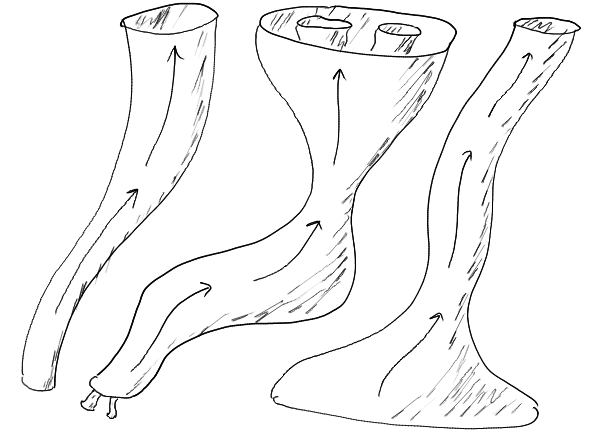
\includegraphics[width=\linewidth]{mass_tubes2.png}\\
  \centering\footnotesize Two-dimensional representation of tubes of a
  closed outer-oriented 3-form $\yr$
\end{wrapfigure}
visualized in spacetime as a set of uninterrupted tubes possessing a
definite orientation along them. The tubes are chosen by us: if we select a
closed two-dimensional surface on a spacetime slice, where $\yr \ne 0$, the
matter 3-form selects a unique tube with 3-dimensional section containing
that 2-surface. This represents our ability to mark a small body of matter
-- say, by drawing a \enquote{$\mathord{\bigcirc}$} sign on an body, or
throwing some leaves in flowing water -- and then to follow it as it moves
and deforms in space as time passes, with respect to some slicing and
frame. A closed outer-oriented 3-form is the perfect mathematical
representation of this.

Note that by \enquote{matter} I mean something which possesses mass, and
I'm thus excluding the electromagnetic field, for example, which is often
considered as matter in general relativity.

If we were to include a theory
of mixtures \citep[\eg][app.~5B]{truesdell1969_r1984}, we would represent
different substances by different matter 3-forms, which could also coexist
in the same spacetime region.


The matter 3-form $\yr$ provides a frame $\yn$ wherever it doesn't vanish.
It is called a Lagrangean or \emph{material} frame
\citep{smarretal1978,smarretal1980} and defined by
\begin{equation}
  \label{eq:eulerian_frame_conditions}
  \yn \cdot \yr = 0, \qquad \yn \cdot \di t = 1.
\end{equation}
It represents the correspondence of places at different times defined by
simply saying that each part of that body is at rest. Note that $\yn$ is
not the 4-velocity of matter; the latter is given by the condition
$\yn\cdot \di\ytn = 1$ in Newtonian relativity and
$\abs{\yn\cdot\yfg\cdot\yn} = 1$ in general relativity. A matter 3-form
cannot be used to define time lapse or distance, owing to its purely
differential-geometric nature.

The matter 3-form of a body can also be used to define a volume element on
each slice, by decreeing that each unit of mass of that body occupies a
unit volume.

Once we have a slicing $t$ and a frame $\yF$, we can project the matter
3-form:
\begin{equation}
  \label{eq:project_matter_form}
  \yj \defd  -\Hat{\yr} \equiv -\yF\cdot\yr,
  \qquad
  \yd \defd \widebar{\yr} \equiv \yr - \di t \land (\yF\cdot\yr).
\end{equation}
We can speak of the amount of matter contained at time $t$ within a
3-dimensional region on a slice: it's the integral of $\yd$ (or $\yr$) over
that region. We can speak of the rate at which matter is flowing through a
stationary outer-oriented 2-dimensional surface on a slice: it's the
integral of the outer-oriented 2-form $\yj$ over that surface. We can also
speak of the spacelike velocity of matter with respect to the frame $\yF$
at time $t$: it's the vector $\yvt$, tangent to the slice, satisfying
\begin{subequations}
  \label{eq:matter_velocity_in_frame}
  \begin{gather}
    \yvt \cdot \di t = 0, \qquad
    \yvt \cdot \yr = - \yF \cdot \yr
    \quad\text{or}\quad
    \yvt \cdot \yd = \yj,
    \\
    \shortintertext{or equivalently, in terms of the Eulerian frame~\eqref{eq:eulerian_frame_conditions},}
    \yvt \defd \yn-\yF;
  \end{gather}
\end{subequations}
\ie\ it's the difference between the frame $\yF$ and the Eulerian frame
$\yn$. This is a velocity in the sense of our convention of slicing \amp\
frame, not in the metric sense. For the latter, we would have to replace
the left \eqn~\eqref{eq:eulerian_frame_conditions} with a normalization
condition.

The outer-oriented 3-form $\yd$ is a density when it's restricted to a
slice. It corresponds to \enquote{$\rho\di\bm{\tau}$}, where
\enquote{$\rho$} is mass density (mass/volume) and {$\di\bm{\tau}$} a
volume element. Thus its unit of measure is mass. The outer-oriented 2-form
$\yj$ is related -- but doesn't correspond -- to \enquote{$\rho\bm{v}$},
where {$\bm{v}$} is the traditional velocity (length/time). This product is
the traditional momentum, which is identical with mass flux in continuum
mechanics. But, as we'll see, we have to  keep these two notions distinct.
The 2-form $\yj$ is mass-flux, but not momentum.

With the projections~\eqref{eq:project_matter_form} and the expression for
the differential~\eqref{eq:d_projection}, the mass
balance~\eqref{eq:mass_density_closed_three_form} can be expressed as
\begin{equation}
  \label{eq:mass_balance_traditional}
  \Li_{\yF}\yd + \di\yj = 0,
\end{equation}
since $\di\yd\equiv 0$ on a slice by construction. This simple, metric-free
formula should be compared with the one involving the covariant derivative
or several metric volume elements when matter flow is expressed by a
1-vector or a 1-form instead \citep[\eg][\eqn~(7.205), \sect~7.3,
p.~361]{rezzollaetal2013}.

By specifying a slicing, a frame, and a matter 3-form, we are specifying a
differential-geometric kinematics. We're only short of a time lapse and a
distance for a kinematics in the traditional sense. The major aim of
Newtonian relativity is to specify the causes that lead to a particular
kinematic.

\medskip

We have here pulled the following piece of thread: mathematically defining
mass as a three-form, with its
conservation~\eqref{eq:mass_density_closed_three_form} or
\eqref{eq:mass_balance_traditional}. This seems to be most natural and
convenient: metric-free and valid in both Newtonian and general relativity.
The tangled bundle loosens here.

But alas, it gets more tangled elsewhere. The projection $\yj$ of the
matter 3-form on the frame,
\eqn~\eqref{eq:project_matter_form}\textsubscript{left}, is a 2-form, and
traditionally it would be considered as \enquote{momentum}. As momentum it
would be part of the energy-momentum-stress tensor $\yTf$, which has order
2. This only works if we represent it as a \emph{1}-form or a vector.
Should we change our representation of the energy-momentum-stress tensor
$\yTf$ then, to something of a different order? We'll see in \sect** that
there are other reasons to do so indeed. But in Einstein's equations
$\yG = 8\pu\yTf$ this tensor is equated to the Einstein tensor $\yG$; thus
we would need to find a different representation of the latter, too.


\iffalse Question: would the notions and objects just introduced suffice for a
kinematic of bodies in spacetime? If the laws that determine their mutual
motions didn't need metrics or parallel transport, wouldn't the topological
description above be enough? I don't think this is a completely idle
question; it isn't yet clear to me which are the experimental operations in
which metric is indispensable. Forces are often dependent on metric
variables, and so metric seems to be tied with dynamics; but how much is it
tied with kinematics? One could say: \enquote{if you throw an apple in the
  air, its motion is described by a parabola, and this fact is important if
  you want to predict where the apple will land}. That's true, but I can
also say that it is a parabola with respect to the Earth and its atmosphere
considered as a round body, or to my arms considered as rigid straight
segments. Thus the notion of distance apparently needed in the description
of the apple's motion seems to be a result of \emph{decreeing} some bodies
around us to be rigid and to have particular shapes. In a relative
description of motion, distance doesn't seem to be necessary.
\fi



\section{Force in Newtonian relativity}
\label{sec:force}




The second piece of thread we're going to pull is \emph{force}. This is
actually a smaller bundle in itself, and we'll examine it from several angles.

***why no need to speak of conservation

***dynamics comes from stating that the total force and total torque vanish

***affine structure needed, related to Newton's 3rd law. But if we assume
only contact forces, it can be expressed locally without parallel
transport. Exception: add spacelike surfaces from a 4D point of view

***that would suffice. But 1st law of thermodynamics, needed for
thermomechanics, mixes force in energy equation as work.

***can there be force where there's no mass? And where there's no EM field?

***when the constitutive equation for a force \enquote{visibly} depends on
space or time variables, as is the case for elastic or inertial forces, the
amount of work done by the force can be \enquote{read} in a change of that
variable. This change is usually called \enquote{energy}. Typical examples
are elastic force $-kx$ and elastic energy, the integral of $-kx\Dot{x}$
being equal to $-\frac{1}{2}kx^2$ no matter how $x$ depends on time; and
inertial force $-m\ddot{x}$ and kinetic energy, the integral of
$-m\ddot{x}\Dot{x}$ being equal to $-\frac{1}{2}m\Dot{x}^2$ no matter how
$x$ depends on time. For viscous forces like $-\eta\Dot{x}$ we usually
don't speak of \enquote{viscous energy} probably because the integral of
$-\eta\Dot{x}^2$ does not have a closed form. This fact is obviously
related to the difference between conservative and non-conservative forces
and to the existence of potentials.

\subsection{Constitutive equations}
\label{sec:constit_eq}



\subsection{Geometric representation}
\label{sec:geometry_force}

In most presentations of the Newtonian mechanics of point masses, force is
represented as a vector bound to a point mass. If we take the line integral
of this vector along the trajectory of the point mass, we obtain the work
made by the force on the mass. In continuum mechanics this picture becomes
more complex. We deal with extended bodies, and the total force on a body
or on part thereof is obtained by integrating two kinds of forces:
\emph{bulk forces}, also called body forces, which act on a mass or volume
element and must be integrated over a three-dimensional region, and
\emph{surface forces}, also called contact forces, which act on an area
element of the body's surface and must be integrated over a two-dimensional
region.

Let's see what kind of geometric representation these operations suggest.

The fact that a force is to be integrated over a line to obtain work
suggests that it's better viewed as a \emph{covector-valued} object, ready
to be integrated over a line without the need of a scalar product
\cites[\sect~12]{burke1995}[\sect~VII.2]{schouten1951}[\sect~2]{vandantzig1954}[\chaps~VI--VII]{burke1985_r1987}[\chap~7]{bambergetal1988_r1990}.
Let's adopt this representation for the moment, although we'll see later
that a different one may be more appropriate.

If a bulk force is to be integrated over a volume, then it should be a
covector-valued, outer-oriented 3-form. If we think of it as operating on a
mass element (outer-oriented 3-form) instead, then it should be a
covector-valued, outer-oriented 3-vector. Here we see the core of one of
the questions of \sect~\ref{sec:soup}: are we to interpret forces as
\enquote{acting} on matter? or as entities that can exist where there's no
matter? General relativity suggests the latter interpretation. But we'll
see that we can bypass the question of this representation in general
relativity, because the notion of bulk force disappears there, leaving only
that of surface force.

Surface forces, being integrated over a surface, should be covector-valued,
outer-oriented 2-forms.

The integration of bulk or surface forces, which are covector-valued
object, is possible in Newtonian mechanics thanks to the affine structure of
its three-dimensional space. This kind of integration is impossible or
at best ambiguous with the path-dependent parallel transport of general
relativity; this impossibility is related to the absence of a
\enquote{conservation law} for 4-momentum \cites[\sect~21]{pauli1921_t1958}[\sect~59]{eddington1923_r1930}[\sect~96]{landauetal1939_t1994}[also][]{aldermanetal1970}.


**1-form also suggested by principle of virtual work

\subsection{Frame indifference}
\label{sec:frame_indifference}


\subsection{Work and frames}
\label{sec:work_frames}


\subsection{Inertia as force and affine structure}
\label{sec:inertia_is_force}

*** only affine structure is necessary to transport and sum forces

*** static formulation  \citep[\cf][\sect~6, p.~652]{vandantzig1934d}

\subsection{Bulk and surface forces}
\label{sec:surface_forces}

\subsection{Four-dimensional generalizations}
\label{sec:4D_generalize}

*** 4th component, spacelike 3-surface


\subsection{Newtonian relativity}
\label{sec:newtonian_mechanics_aim}

The main aim of continuum mechanics is to describe how bodies move and
deform in spacetime in response to forces. 

In the history of science we see two main kinds of scientific theory.

One kind of theory is based on the \enquote{stuff} that is believed to be
ultimate and fundamental at the time of conception, although usually proven
not to be ultimate some decades later. Examples are vortex theories from
the Baroque and contemporary high-energy particle theories.

The other kind of theory, humbler and more grandiose at the same time,
tries to make allowance for any new phenomena that may be discovered.

Newtonian thermomechanics belongs to the second kind. Its aim is not to
describe this or that particular particle or field, or this or that
fundamental interaction. Its purpose is the description, within particular
ranges and resolutions of space and time, of any kind of material and
substance that humans use now or will discover in the future. For this
purpose it uses some concepts devised, with their generality, to be able to
accommodate as many new phenomena as possible. The main one is the concept
of force.

Our exploration cannot only be based on mathematical manipulation of the
Einstein equations, but also requires a clear view of the way continuum
thermomechanics is used. % General relativity, having being conceived at
% the same time as the great quantum and particle discoveries were made,
% was greatly influenced by the latter in its use, despite being much more
% akin in spirit and mathematics to Newtonian continuum mechanics.

Newtonian continuum thermomechanics, which I'm here calling
\enquote{Newtonian relativity}, has been refined under more than 300 years
and has today a crystal-clear, yet far from finished, method and structure:
\begin{itemize}[para]
\item Its purpose is the description, within particular ranges and
  resolutions of space, time, energy, of any kind of material or substance
  that Man uses now or will discover in the future. This must be contrasted
  with contemporary particle high-energy physics, whose goal is the
  description of \emph{only} those forces and kind of matter believed to be
  \enquote{ultimate}. The scope of Newtonian continuum thermomechanics is
  from this point of view wider than that of particle physics.
\item For this description it uses five fundamental balance laws and a set
  of nine physical quantities:
  \begin{itemize}
  \item balances: mass, force, torque, energy, entropy;
  \item quantities: mass, displacement, temperature, stress,
    internal energy, heating flux, entropy, body force, body heating.
  \end{itemize}
  The quantities and balances above are postulated to apply to any kind of
  matter or substance. Mass, displacement, temperature are independent
  quantities. Body force and body heating must be given in any particular
  problem and express the effect of the surroundings The remaining are
  dependent quantities.
\item Each particular kind of matter, with its different behaviours and
  responses, is characterized by a set of \emph{constitutive equations}.
  These equations express the particular dependence of the dependent
  quantities on the independent ones, and together with the balances and
  initial and boundary conditions yield a well-posed system of
  integro-differential equations. Specifically, the constitutive equations
  give stress, internal energy, heating flux, and entropy as functionals of
  mass, displacement, temperature. The difference between al kinds of
  liquids, gases, solid, plasmas resides in the constitutive equations.
  
  Sometimes internal energy is taken and independent, and temperature as
  dependent with an appropriate constitutive equation.
\end{itemize}

The separation of balance laws and constitutive equations is fundamental
and reflects the aim of continuum mechanics to describe \emph{any} kind of
force and matter that can be discovered, not just those that our century
believes to be the only existing ones. We can make a parallel with
Hamiltonian mechanics: Hamilton's general equations correspons to the
balance laws; particular Hamiltonians correspond to particular constitutive
equations.



\section{Newtonian-relativistic continuum mechanics: kinematics}
\label{sec:newton_kinematics}


\section{Newtonian-relativistic continuum mechanics: dynamics}
\label{sec:newton_dynamics}

\subsection{Dynamics with absolute time}
\label{sec:newton_dynamics_absolute_time}

Traditional presentations of Newtonian-relativistic dynamics and of
Newton-Cartan theory starts with the notion of \emph{absolute time} $\ytn$,
which is a unique slicing of spacetime. We'll presently see that this
notion, together with a geometry and a connection on the slices, is
mathematically necessary when the notion of force is represented by objects
living on 3-surfaces. But later we'll consider the possibility of avoiding
absolute time. In fact, the notion of simultaneity in
Newtonian-relativistic mechanics is inspired by what we simultaneously
\emph{see}, together with the assumption that the velocity of light is
practically infinite. But we could also define simultaneity in terms of
what we simultaneously \emph{hear}, for example. How could Newtonian
mechanics be formulated in that case? We'll give a possible answer later.

A force on a body at time $\ytn$ in Newtonian mechanics has two important
characteristics:
\begin{enumerate*}[label=(\arabic*)]
\item it is meant to be integrated along the trajectory of every small
  region of the body, to yield the work done on that region;
\item it is meant to be obtained from the sum of infinitesimal body forces
  acting over each part of the region, or surface forces over its boundary.
\end{enumerate*}

Owing to the first characteristic, many geometers
\citep{vandantzig1954,burke1980b,burke1985_r1987,burke1995,bossavit1991,bossavit1998b,hehletal1999,hehletal2003}
have advocated the representation of force as a covector. Their arguments
are valid and geometrically beautiful, and therefore we assume for the
moment that forces are covector-valued objects.

Note, however, that the covector-valued conception of force is
geometrically unsatisfying, because velocity is a frame-dependent object.
Later on I will use a frame-indifferent notion more primitive than
velocity.

The second characteristic says that a body force must be a covector-valued
outer-oriented 3-form, while a surface force a covector-valued
outer-oriented 2-form.

The total force on a body is the integral of the body forces over its
volume and of the surface forces over its boundary. Since forces are
vector-valued objects, this integration is only possible if the slices
have an \emph{affine} structure, that is, a parallel transport with
vanishing curvature. From this point of view, the affine structure is
demanded by the dynamics, rather than by the kinematics.

Some forces between bodies, like the gravitational force or a purely
elastic stress, are moreover defined to depend on a metric, which must
therefore be introduced besides the affine structure. It would be
interesting to explore whether metric and affine structure could be
introduced in terms of these forces instead.

So in the present section let's assume that we have a unique slicing
$t\equiv\ytn$, representing absolute time, and whose slices have a
Euclidean structure: metric $\yg_t$ and flat parallel transport $\ynab_t$;
the index $t$ will be omitted, but it is important to note that there is no
specific relation between metrics and parallel transport on different
slices. We are not assuming the existence of a Newton-Cartan connection. A
frame $\yF$ that satisfies $\Li_{\yF}\yg = 0$ is called a \emph{rigid
  frame}.

Indicating the sum of all body forces acting on a body by $\yb$, and that
of the surface forces by $\yT$, the \emph{balance of forces} states that
\begin{equation}
  \label{eq:force_balance_integral}
  \int_{\yvo} \yb + \oint_{\de\yvo} \yT = 0 \qquad\forall \yvo
\end{equation}
for each outer-oriented closed 3-volume $\yvo$ within a slice. Note that the
result of the integration is a 1-form, not a scalar. The local version of
the balance is
\begin{equation}
  \label{eq:force_balance_ecd_local}
  \yb + \yDi \yT = 0, 
\end{equation}
where $\yDi$ is the \emph{exterior covariant derivative}
\cites[\sect~Vbis.A.4]{choquetbruhatetal1977_r1996}[\sect~14.5]{misneretal1970_r2003}[\sect~9.3]{frankel1997_r2012}[see
also][]{segev2000,segev2000b,segevetal2000,segev2002,segevetal2012,kansoetal2007}.

The fact that we have to use the \emph{exterior} covariant derivative, rather than
the covariant derivative, may have important consequences later.

\subsection{Interlude: forces and motion -- is there a balance of
  momentum?}
\label{sec:really_balance_momentum}

How does the balance of forces relate to motion?

The vast majority of literature and textbook do not speak of balance of
forces; they follow a different path that sounds more or less as follows:

There is a law of \enquote{conservation of momentum}, which states that the
rate of change of momentum of a body region is proportional to the forces
exerted on it:
\begin{subequations}\label{eq:conservation_momentum_traditional}
  \begin{gather}
    \label{eq:conservation_momentum_traditional_integral}
    \text{\textquotedblleft}\ 
    \di_t\int_{\yvo}\yd\yvt = \int_{\yvo} \yb + \oint_{\de\yvo} \yT
    \ \text{\textquotedblright},
    \\\shortintertext{or}
    \label{eq:conservation_momentum_traditional_differential}
    \text{\textquotedblleft}\ 
    \de_t(\yd\yvt) + \div(\yd\yvt\otimes\yvt) = \div\yT +\yb
    \ \text{\textquotedblright}.
  \end{gather}
\end{subequations}
This equation directly connects forces and motion, and looks like a
conservation equation with fluxes and sources. This conservation law is
only valid in an inertial frame. We can make it valid in every rigid frame
provided we add some \enquote{fictitious forces} looking like
\begin{equation}
  \label{eq:fictitious_forces}
    \text{\textquotedblleft}\ 
  \yd\, [-{\de_t}^2\yxto%(\yxt-\yxto)
  + 2\yom\cdot\de_t(\yxt-\yxto) + (\de_t\yom-{\yom}^2)\cdot(\yxt-\yxto)]
    \ \text{\textquotedblright},
\end{equation}
in that non-inertial rigid frame.

\bigskip

The presentation above is geometrically unsatisfying, however.

The right-hand side of \eqn~\eqref{eq:conservation_momentum_traditional} is
frame-indifferent; that is, the definition and measurement of $\yT$ and
$\yb$ do not depend on a choice of frame, inertial or otherwise. For
example, the force exerted on a pointlike object attached to a Hookean
spring with constant $k$ and elongation $l$ has intensity $kl$ and
direction along the elongation. This is a complete description of the
force, and the notion of frame is completely irrelevant to it. Similarly
for the gravitational force: it is given by $\yd\otimes\yfg$, where $\yfg$
is a frame-indifferent covector field. This field is in turn determined by
the mass distribution via $\di\yfg = - 4\pu G \yd$, again a
frame-indifferent definition.

The momentum density $\yd\yvt$ on left-hand side of
\eqn~\eqref{eq:conservation_momentum_traditional} and the
\enquote{fictitious forces}~\eqref{eq:fictitious_forces} require the
specification of a frame instead.

Therefore \eqn~\eqref{eq:conservation_momentum_traditional}, with or
without fictitious forces, mixes up frame-indifferent and frame-dependent
quantities. This doesn't make sense geometrically.

We find a geometrically more satisfying formulation by using some ideas
that can possibly be found in a work by Jacob Bernoulli
\citey{bernoulli1703} \citep[see][p.~104]{truesdell1968}  \cites{noll1963}[\sect~I.13]{truesdell1977_r1991}. Consider a small
enough body region, so that deformation and torques can be neglected. In a
problem of \emph{statics} in an inertial frame, the balance of
forces~\eqref{eq:force_balance_integral} holds. Now consider a fact and two
assumptions:
\begin{itemize}
\item a small body region can always be considered at rest in a suitably
  chosen frame;
\item the laws of statics should hold in any frame in which the body region
  is at rest;
\item an inertial frame is a rigid frame at rest on average with respect to
  the total distribution of matter in the universe, which is mostly
  associated with the fixed stars.
\end{itemize}
The consequence of these statements is that \emph{the balance of
  forces~\eqref{eq:force_balance_integral} is valid in any frame; among
  these forces we must account for one related to the relative motion of
  the body region with respect to the total distribution of matter in the
  universe, approximately identified with the \enquote{fixed stars}}.

This force is the inertial force. Let's see how it is expressed in an
arbitrary rigid frame $\yF$; remember that what we call \enquote{time
  derivative} is the Lie derivative $\Li_{\yF} \defs \de_t$. In this frame
let the position of the body region be $\yxt(t)$, and let the total
distribution of matter in the universe have centre of mass at $\yxto(t)$
and average instantaneous rotation given by the 2-form $\yom(t)$; in
\sect~\ref{sec:inertial_force} I explain how they are determined by the
mass distribution through a sort of Mach's principle. Then the inertial
force is the covector-valued 3-form
% \begin{equation}
%   \label{eq:inertial_force}
%   \ybi \defd  -\yd\, [{\de_t}^2(\yxt-\yxto)
%   - 2\yom\cdot\de_t(\yxt-\yxto) - (\de_t\yom-{\yom}^2)\cdot(\yxt-\yxto)].
% \end{equation}
\begin{equation}
  \label{eq:inertial_force}
  \ybi \defd  -\yd \otimes
  \bigl(\yom\cdot\yg^{-1}\cdot\yom  - \de_t\yom - 2\yom\de_t  + \yg{\de_t}^2\bigr)
  \cdot(\yxt-\yxto).
\end{equation}
The definition of this force requires a metric on each slice. The definition
of its source, see \sect~\ref{sec:inertial_force}, also requires a parallel
transport on each slice. But it does not require a 4-dimensional connection
on the whole spacetime. If we choose a rigid frame in which the total
matter of the universe does not rotate on average, $\yom=0$, and moves with
uniform velocity, $\de_t\yxto=\text{const}$, then we recover the familiar
expression $\ybi = -\yd \yg\cdot{\de_t}^2\yxt$ -- the $\yg$ is necessary to
transform a vector into a covector. This kind of rigid frame is called
inertial. The use of a \emph{rigid} frame is not necessary; a
frame-independent expression of the inertial force is given below.

Including the inertial force in the sum of all other body forces $\yb$, the
balance of forces~\eqref{eq:force_balance_integral} includes the familiar
Newtonian equations of motion. It is the inertial force that in most
physical situations links kinematics and dynamics, specifically by linking
forces upon a body to its motion with respect to the rest of matter in the
universe. But there are also situations in which inertia is inessential.
For example, consider a small body of negligible mass attached to a Hookean
spring inside a fluid, the other end of the spring being at rest with
respect to the fluid. The forces acting on the body are the Hookean and the
viscous ones. In a suitable frame of reference the balance of forces is
$-k\yxt - \eta\de_t\yxt = 0$, leading to a specific motion
$\yxt(t) = \e^{-kt/\eta}\yxt(o)$ with respect to the fluid. In this example
the inertial force plays no role and it is not important whether the frame
is inertial or not.

As regards \enquote{conservation of momentum}, we see that the
time-derivative of momentum in Newtonian mechanics is not a quantity with a
general geometric meaning: it is the simplified form assumed by a
particular force in a particular frame. From this point of view
conservation of momentum is not a general geometric notion in
Newtonian-relativistic mechanics.




The inertial force on the mass $\yr$ can be written in a frame-free way as
$-\yg^{-1}\cdot \Li_{\yFi}(\yFi\cdot\yr)$, where $\yFi$ is a vector field
transverse to the slices, defined in \sect~\ref{sec:inertial_force}. Some
forces, like inertial, viscous, and electromagnetic ones, require objects
transverse to the slicing for their definition, whereas others, like
elastic or gravitational ones, don't. This suggests that the presentation
in terms of an absolute-time slicing can be geometrically improved upon.


\subsection{Balance of energy}
\label{sec:energy_balance}

To each matter element on each slice is also associated an internal energy
density $\ye\yd$, represented by an outer-oriented 3-form proportional to
the mass 3-form $\yd$. The balance of energy states that the change in the
total energy in a 3-volume $\yvo$ on a slice must come from the energy
transported thither or thence, from the work done by the forces, and from
body and surface heating, represented by outer-oriented 3-form and 2-form:
\begin{equation}
  \label{eq:balance_energy_traditional}
%   \de_t \int_{\yvo}\ye =
%   \int_{\yvo} \yvt\cdot\yb + \oint_{\de\yvo} \yvt\cdot\yT
% +  \int_{\yvo} \yQ + \oint_{\de\yvo} \yq
%   \qquad\forall \yvo
%  \\
%  \shortintertext{or}
  \de_t(\ye\yd) + \di(\yvt \cdot \ye\yd) =
  \yvt\cdot\yb + \di(\yvt\cdot \yT)
  +\yQ + \di\yq,
\end{equation}
with $\de_t(\ye\yd) \equiv \Li_{\yF}(\ye\yd)$. The rate of change of
kinetic energy is simply the work done by the inertial force, and is
therefore included in the term $\yvt \cdot \yb$. The traditional expression
with \enquote{$\de_t + \yvt\cdot\ynab$} appears if we write the 3-form
$\ye\yd$ as a multiple of the volume element $\ygv$ -- one more example of
a unnecessary use of metric.

If we assume that body forces and body heating vanish, then we can rewrite
this equation as
\begin{equation}
  \label{eq:balance_energy_suggests_3form}
  \de_t(\ye\yd) + \di(\yvt \cdot \ye\yd -\yvt\cdot\yT - \yq) = 0,
\end{equation}
which suggests that energy can also be considered like an outer-oriented
closed 3-form, with a flux 2-form
\begin{equation}
  \label{eq:energy_4velocity}
  \yp \equiv -\yvt \cdot\ye\yd + \yvt\cdot\yT +\yq.
\end{equation}


\subsection{Constitutive equations}
\label{sec:constitutive equations}

\mynote{This section is disconnected from the rest. To be rewritten}

The balances of mass, force, energy give a system of 1+3+1 real-valued
equations. They involve at least 4+3+6+5 real-valued components: mass
density and flux, body force and stress, energy density and flux, and body
supply of energy. The independent variables in these equations are usually
assumed to be the four components of the mass 3-form -- that is, mass
density and mass flux or velocity -- and the temperature. Sometimes the
energy density is exchanged with the temperature in the role of independent
variable.

The balance laws alone are therefore not sufficient to determine the
evolution of all fields. Moreover, although the balances are assumed to
hold for all forms of matter, different kinds of matter behave in different
ways.

\emph{Constitutive equations} are equations that gives the dependent fields
as functions or functionals of the independent ones. They express the
different behaviours of different kinds of matter, and together with the
balance laws yield a closed system of differential or integro-differential
equations.

The most important constitutive equation in our discussion is that for the
4-stress. All 4-components of the stress $\yT$ are in the simplest cases
functionals of the mass 3-form $\yr$, the internal energy $\ye$ or
temperature $\yte$, and the 3-metrics $\yg$:
\begin{subequations}\label{eq:constitutive_4stress}
  \begin{gather}
    \label{eq:constit_T_with_mass_geometry}
    \yTf=\yTf(\yr,\yte,\yg),
    \\
    \shortintertext{or, in a given slicing and frame,}
    \label{eq:4stress_components}
    \yTf =
    \begin{pmatrix}
      \ye(\yd,\yj,\yte,\yg) & \yq(\yd,\yj,\yte,\yg) \\
      \yp(\yd,\yj,\yte,\yg) & \yT(\yd,\yj,\yte,\yg)
    \end{pmatrix}.
  \end{gather}
\end{subequations}
The dependence on the metrics can be complicated: for example, the stress
at a point can depend on the difference between the 3-metric there and the
metric from previous 3-surfaces, transported by the velocity $\yc$
associated with the mass flux\citep{grotetal1966,carteretal1972}. The
difference can be non-vanishing even if the 3-metric is Euclidean on all
3-surfaces. The only difference between Newtonian and general relativistic
mechanics is that all 3-metrics are flat in the former but not in the
latter.


\subsection{Dynamics without absolute time}
\label{sec:newton_dynamics_without_absolute_time}

The formulation of dynamics of
\sect~\ref{sec:newton_dynamics_absolute_time} has the advantage of being
frame-indifferent: inertial frames don't have a special status, and inertia
is just one force among many others. But that formulation still has several
interrelated unpleasant features:
\begin{itemize}
\item a special absolute-time slicing is used,
\item forces, energy, energy fluxes are only defined on the slices of that
  slicing,
\item forces are meant to act on velocities, which are frame-dependent,
\item a flat parallel transport is needed to integrate the forces.
\end{itemize}

A first step in lifting forces from their plain existence on slices to a
fourfilling existence in spacetime, and in unchaining them from
frame-dependent velocities, is to assume that they act directly on the
four-dimensional mass flux expressed by the matter 3-form. This requires
that they have \emph{outer-oriented 3-vector} values. It also means that
their physical dimension acquires a $[\text{mass}^{-1}]$ factor.

A 3-vector has four components. The additional component of a force is
interpreted, both in Newtonian \cites[\sects~152--154,
288--289]{truesdelletal1960}[\sect~2.3]{grotetal1966} and Lorentzian
\cites{eckart1940c}[\sect~2.3]{grotetal1966}{maugin1978b} relativity, as
the combination of power and heating. Thus we arrive at the notion of
\emph{heating-force} tensor, which corresponds to the \enquote{four-force}
of Lorentzian relativity.

In this new point of view a surface force -- 4-stress -- is a
outer-oriented-3-vector-valued outer-oriented 3-form. Contracted with a
matter 3-form it yields another outer-oriented 3-form, which could be
interpreted as the spacetime flux of some quantity. From general relativity
we foresee that this quantity is the energy flux.

\mynote{To be added: formulation with 2-point energy-momentum-stress tensor \citep[\sect~288]{truesdelletal1960}}

\subsection{Decoupling force from body}
\label{sec:decoupling_force_body}

In Newtonian relativity, force is something experienced by a body, rather
than something in spacetime. But there are signs that forces need to be
decoupled also in Newtonian relativity.


\subsection{An interesting development?}
\label{sec:interesting_development}


This leads to some interesting developments. Interpret a 4-stress $\yTf$ as
an object which contracted with a matter 3-form $\yr$ yields its
corresponding energy-flux outer-oriented 3-form $\yE$:
\begin{equation}
  \label{eq:stress-matter-momentum}
  \yE = \yTf \cdot \yr.
\end{equation}
This is similar to the \enquote{$^{\displaystyle *}\yTf$} of Misner \etal\
\citep[\chap~15]{misneretal1970_r2003}, with the difference that $\yTf$ is
3-covector valued.

Now postulate that energy flux must always be conserved,
\begin{equation}
  \label{eq:conserv_energy-momentum_try}
  \di\yE = 0.
\end{equation}
We obtain a set of two balances and a relation between them:
\begin{equation}
  \label{eq:massb_energyb_relation}
  \di\yr = 0, \qquad \di\yE = 0, \qquad \yE = \yTf \cdot \yr.
\end{equation}
Question: does this system \emph{imply} Einstein's equations? The point
is that we can now introduce a four-dimensional exterior covariant
derivative $\yDi$ and combine the  equations above as follows:
\begin{equation}
  \label{eq:why_4stress_zero}
     \di\yE
    = \di(\yTf \cdot \yr) 
    = \yDi\yTf \cdot \yr - \yTf \cdot \di\yr
   = \yDi\yTf \cdot \yr
    = 0
\end{equation}
and \emph{asking this to hold for every $\yr$}, we have
\begin{equation}
  \label{eq:div_T_vanishes}
  \yDi\yTf = 0,
\end{equation}
which corresponds to Misner \etal's
\enquote{$\bm{\mathsf{d}}{}^{\displaystyle *}\yTf=0$}
\citep[\chap~15]{misneretal1970_r2003}.

This point of view seems to say that \emph{any exterior covariant
  derivative $\yDi$ will do} -- possibly with additional restrictions
coming from restrictions on positivity of mass and energy fluxes. Such a
possibility is not so strange when we consider that Einstein's equations
can be rewritten, in a completely equivalent way, in terms of a flat
connection with non-vanishing torsion, or a mixture of the two
\citep{deandradeetal2000,arcosetal2004,aldrovandietal2013,pereira2014,caietal2016}.
It seems that what's fundamental here is the use of a derivation operator
with the properties of an \emph{exterior} covariant derivative, rather than
the use of a covariant derivative or parallel transport per se.

Finally, Einstein's equations $\yEi = \yTf$ could simply be interpreted as
\emph{the most general integral of the equation $\yDi\yTf = 0$}. This
possibility is related to an interesting remark by Truesdell:
\begin{quote}
  When the field theories were discovered in the eighteenth century, solutions
in arbitrary functions such as those presented in this subchapter were sought
earnestly, but, for the most part, sought in vain. In the nineteenth century,
researches on partial differential equations turned away from such general
solutions so as to concentrate upon boundary-value problems. When, in the
twentieth century, the general solutions were at last obtained, scarce attention
was paid to them, and to this day they remain virtually unknown. Though
so far they have been used but rarely, they might turn out to be illuminating
in studies of underdetermined systems, where the conventional viewpoint of
partial differential equations has gained little.  \citep[p.~594]{truesdelletal1960}
\end{quote}

\mynote{To be added: refs to Finzi, Beltrami}

\mynote{To be added: discussion about pp.~18--19 of \citep{weatherall2017}:
  use differential forms for Gauss-Green theorem, instead of covariant
  derivative}



\section{General relativity}
\label{sec:general_relativity}

\subsection{Aims}
\label{sec:aims_general_rel}

General relativity gives us the equation $\yG=\kappa\yTf$; for some time
after its proposal it was not clear which were independent, dependent, and
boundary-condition quantities; a distinction that is necessary to set up a
well-posed boundary-value problem. Misner \etal\
\citey[\chap~21]{misneretal1970_r2003} discuss this question at length.

The Einstein equations are clearly suited for a continuum description of
matter, not a particulate one: because they involve the notion of stress,
which is an exquisitely continuum notion. And since stress is the staple of
constitutive equations in Newtonian mechanics, and does not commit to
specific forms of matter or forces, then the Einstein equations do not
commit to specific forms of matter or forces either, unlike
particle-physics theories. From this point of view the Einstein equations
appear as a harmonization of a part of the Newtonian balance laws and of
geometry. They -- especially the stress appearing in them -- still need
constitutive equations.

The Einstein equations don't include the balances of mass and entropy
\cites{eckart1940c}[\chap~22]{misneretal1970_r2003}. This fact is very
clear in numerical relativity
\cites[p.~1918]{disconzi2014}[\sect~2.2]{wilsonetal2003_r2007}[\sect~6.3.2]{gourgoulhon2007_r2012}[\chap~5]{baumgarteetal2010}[\sect~2.3]{rezzollaetal2013}.


 
\subsection{3~+ 1 formulation}
\label{sec:3-1_formulation}

Spacetime can be sliced and a frame introduced just like in the Newtonian
case of \sect~\ref{sec:slicing_frames}.

The Einstein equations can be decomposed by projection along the slices $t$
and the frame $\yn$, giving rise to a part parallel to the surfaces with
3\;\texttimes\;3 real components, a part parallel to the vector field with
1 component, and a mixed part with 3 components. Our freedom in choosing
the slicing $t$ and the frame $\yn$ appears in the decomposed equations
as the presence of and undetermined \enquote{lapse} function and an
undetermined \enquote{shift} vector field. When a metric is present we can
choose the frame $\yn$ to be the unit normal to the 3-surfaces. This choice
corresponds to a constant unit lapse function and a vanishing shift vector
\citep{smarretal1978,smarretal1980}. Other choices of lapse and shift are
more convenient for the initial-value problem, for example because they can
correspond to a slicing that covers most of spacetime while avoiding
singularities \citep{smarretal1978}. But our present discussion is mainly
conceptual; we therefore use the simplest lapse and shift.

The decomposed Einstein equations can be found compactly written in a
number of texts
\cites[\sect~1.3]{wilsonetal2003_r2007}[\sect~4.3.2]{gourgoulhon2007}[\chap~2]{alcubierre2008}[\sect~7.2.2]{rezzollaetal2013}.
The decomposition of the Einstein tensor $\yG$ yields the 3-metric
$\yg=(\ygg_{ab})$ of the 3-surfaces, having inverse $\yg^{-1}=(\ygg^{ab})$,
with its compatible connection $\ynab$ having Ricci curvature
$\yR=(\yRR_{ab})$, and the extrinsic curvature $\yK=({\yKK_a}^b)$ of the
3-surfaces. The decomposition of the energy-stress tensor $\yTf$ yields the
internal energy $\ye$, energy flux $\yp$, and spatial stress
$\yT=({\yTT_a}^b)$:
\begin{equation}
  \label{eq:decomp_4stress}
  \yTf = \ye \di t \otimes\yn + \yp\otimes\yn + \di t
  \otimes(\yp\cdot\yg^{-1}) + \yT.
\end{equation}

The Einstein equations $\yG = 8\pu\yTf$ are decomposed into the evolution
equations
\begin{subequations}\label{eq:evolution_eqns}
  \begin{align}
    \label{eq:dt_metric}
    \de_t \yg &= -2\yK\cdot\yg,
    \\
    \label{eq:dt_curvat}
    \de_t \yK &=  \yK\tr\yK + \yR\cdot\yg^{-1} + 4\pu\,(\tr\yT-\ye) - 8\pu\yT,
  \end{align}
\end{subequations}
and the constraint equations
\begin{subequations}\label{eq:constraint_eqns}
  \begin{align}
    \label{eq:energy_constraint}
    16\pu\ye &= (\tr\yK)^2 - \yK\con\yK + \yR\con\yg^{-1},
    \\
    \label{eq:momentum_constraint}
    8\pu\yp &= \ynab\cdot(\yK\T - \yI\tr\yK).
  \end{align}
\end{subequations}
Note that
\begin{equation}
  \label{eq:curvature_stretching}
  \yK\cdot\yg = -\frac{1}{2}\de_t\yg \equiv
  -\frac{1}{2}  \Li_{\yn}\yg \equiv
  -\frac{1}{\sqrt{\yg}}\Li_{\yn}\sqrt{\yg} \equiv -\ynab\cdot ***
\end{equation}

It is interesting to note that \enquote{3-momentum} in relativity appears
as the divergence of a 3-tensor -- just like the force from a stress.

To these equations we must add the mass balance, equivalent to
\eqn~\eqref{eq:mass_balance_traditional}:
\begin{equation}
  \label{eq:mass_balance_gen-rel}
  \de_t\yd = - \di\yj.
\end{equation}
In these expressions $\de_t \equiv \Li_{\yn}$.

This gives us a total of 6 + 6 + 1 + 3 + 1 real-component equations for a
total of 6 + 6 + 6 + 1 + 3 + 1 + 3 + 1 real components of the fields $\yg$,
$\yK$, $\yT$, $\ye$, $\yp$, $\yd$, $\yj$, and temperature $\yte$. Then we
need 6 + 1 + 3 equations, which turn out to be, as in the Newtonian case,
the constitutive equations~\eqref{eq:constitutive_4stress} for the
energy-stress:
\begin{subequations}\label{eq:constitutive_4stress_gen-rel}
  \begin{align}
    \label{eq:constit_energy_gen-rel}
    \ye &= \ye(\yd,\yj,\yte,\yg, \yK),
    \\
    \label{eq:constit_energy-flux_gen-rel}
    \yp &= \yp(\yd,\yj,\yte,\yg, \yK),
    \\
    \label{eq:constit_3stress_gen-rel}
    \yT &= \yT(\yd,\yj,\yte,\yg, \yK).
  \end{align}
\end{subequations}

\subsection{Parentetical remark: divergence of energy-stress}
\label{sec:divergence_4stress}

A strange point appears in most general-relativity texts I've seen,
especially for numerical relativity. They remark that the balance equations
$\ynaf\cdot\yTf = 0$ are a consequence of the Einstein equations
$\yG = 8\pu \yTf$, and therefore solving the latter automatically yields
the former. But to find the numerical solutions they actually use the
former!

The balance $\ynaf\cdot\yTf = 0$ is indeed contained in
\eqns~\eqref{eq:evolution_eqns}--\eqref{eq:constraint_eqns}. For example,
combining the time derivative of the constraint
equation~\eqref{eq:momentum_constraint} and the 3-divergence of the
evolution equation~\eqref{eq:dt_curvat} we obtain the spatial part of
$\ynaf\cdot\yTf = 0$: the balance of momentum. A quick check of such
combination of \eqref{eq:momentum_constraint} and \eqref{eq:dt_curvat}
shows in fact the appearance of the time-derivative of $\yp$ and the
divergence of the 3-stress. A similar combination yields the balance of
energy:
\begin{subequations}\label{eq:evolution_energy_momentum}
  \begin{align}
    \label{eq:dt_energy}
    \de_t \ye &= \ye\tr\yK - \yg^{-1}\con\ynab\yp + \yK\con\yT
    \\
    \label{eq:dt_momentum}
    \de_t \yp &=  \yp\tr\yK - \ynab\cdot\yT\T,
  \end{align}
\end{subequations}

The reason for using the divergence equation $\ynaf\cdot\yTf = 0$ is
clearly explained by Frittelli \citey{frittelli1997} (the only work I've
found that explains this). The constraint
equations~\eqref{eq:constraint_eqns} should be enforced on \emph{every}
3-surface, \ie\ for all times $t$, while the metric and extrinsic curvature
are evolved by \eqns~\eqref{eq:evolution_eqns}. If we did so there would be
no need to use $\ynaf\cdot\yTf = 0$ in the solution.

But it would be more convenient if the
constraints~\eqref{eq:constraint_eqns} could be enforced on one 3-surface
only, for example the initial one, and be automatically satisfied on all
other 3-surfaces, \ie\ at all subsequent times. It turns out that the
divergence equation $\ynaf\cdot\yTf = 0$ does exactly this: it makes the
constraints automatically satisfied at all times if they are satisfied at
the initial time.

Loosely speaking, the system
\begin{equation*}
  \left\{\begin{aligned}
  &\text{evolution equations~\eqref{eq:evolution_eqns}} \\
  &\text{constraint equations~\eqref{eq:constraint_eqns} for all $t$}
  \end{aligned}\right.
\end{equation*}
is equivalent to the system
\begin{equation*}
  \left\{\begin{aligned}
  &\text{evolution equations~\eqref{eq:evolution_eqns}} \\
  &\text{divergence equation $\ynaf\cdot\yTf = 0$} \\
  &\text{constraint equations~\eqref{eq:constraint_eqns} for initial $t$ only}
  \end{aligned}\right.
\end{equation*}
and the latter is more convenient to solve.


\subsection{How to solve the decomposed equations}
\label{sec:how_to_solve_3-1}

Let us consider how
equations~\eqref{eq:evolution_eqns}--\eqref{eq:constitutive_4stress_gen-rel}
could be solved.

% Only the evolution equations~\eqref{eq:evolution_eqns} and
% mass-balance~\eqref{eq:mass_balance_gen-rel} contain temporal derivatives:
% they give us 6 + 6 + 1 real-components of the $\yg$, $\yK$, $\yd$ fields on
% the 3-surface at time $t+\incr t$ given all fields on the 3-surface at time $t$.
% The constraint equations \eqref{eq:constraint_eqns} and constitutive
% equations~\eqref{eq:constitutive_4stress_gen-rel} fix definite relations
% between metric, extrinsic curvature, energy and energy flux, on each
% 3-surface. The question is which field should be considered independent and
% which dependent.

% In continuum mechanics the stress $\yT$ is in the simplest case a
% functional of mass density, momentum or velocity, and internal energy. For
% the moment let's assume a constitutive equation
% \begin{equation}
%   \yT=\yT(\ye,\yp,\yg,\yK),
%   \label{eq:constit_T_with_energy}
% \end{equation}
% omitting mass density. Then,

Imagining a rough numerical timestepping scheme, in which for example
\eqn~\eqref{eq:dt_metric} becomes
\begin{equation}
  \label{eq:approx_timestepping_dt_metric}
  \yg(t + \incr t) \approx \yg(t) -2\yK(t)\cdot\yg(t)\,\incr t,
\end{equation}
it seems that the
equations~\eqref{eq:evolution_eqns}--\eqref{eq:constitutive_4stress_gen-rel}
can be solved this way:
\begin{enumerate}[leftmargin=1.5\parindent]
\item Choose all fields such as to satisfy the
  constraints~\eqref{eq:constraint_eqns} and constitutive
  equations~\eqref{eq:constitutive_4stress_gen-rel} on an initial 3-surface
  at time $\yto$.
\item\label{item:increase_step}Calculate metric $\yg$, extrinsic curvature
  $\yK$, mass density $\yd$ at time $\yto + \incr t$ from the evolution
  \eqns~\eqref{eq:evolution_eqns} and balance
  \eqref{eq:mass_balance_gen-rel}:
  \begin{align*}
    \de_t \yg &= -2\yK\cdot\yg,
    \\
    \de_t \yK &=  \yK\tr\yK + \yR\cdot\yg^{-1} + 4\pu\,(\tr\yT-\ye) - 8\pu\yT,
    \\
    \de_t\yd &= - \di\yj.
  \end{align*}
  Note that these evolution equations require, in particular, the mass flux
  $\yj$, energy $\ye$, stress $\yT$ at time $\yto$.
\item\label{item:increase_step_energy}Calculate the mass flux $\yj$,
  temperature $\yte$, energy $\ye$, energy flux $\yp$, stress $\yT$ at time
  $\yto + \incr t$ from the system of
  constraints~\eqref{eq:constraint_eqns} and constitutive
  \eqns~\eqref{eq:constitutive_4stress_gen-rel}, given the newly found
  $\yg$, $\yK$, $\yd$:
  \begin{gather*}
    \begin{aligned}
    16\pu\ye &= (\tr\yK)^2 - \yK\con\yK + \yR\con\yg^{-1},
    &\quad
      8\pu\yp &= \ynab\cdot(\yK\T - \yI\tr\yK),
    \\
    \ye &= \ye(\yd,\yj,\yte,\yg, \yK),
    &
      \yp &= \yp(\yd,\yj,\yte,\yg, \yK),
    \end{aligned}\\
      \yT = \yT(\yd,\yj,\yte,\yg, \yK).
  \end{gather*}
  Note that this system \emph{implicitly} yields, in particular, the mass
  flux $\yj$, energy $\ye$, stress $\yT$ needed in the next timestep; see
  step above.

  Now we have all fields at time $\yto + \incr t$.

\item Set $\yto + \incr t \to \yto$, go to step~\ref{item:increase_step}.
\end{enumerate}

It's important to remark that the motion of matter, expressed by the mass
flux $\yj$ in this particular reference frame and slicing, is determined
in an \emph{implicit} way in the scheme above. It would be worth
investigating how geodesic equations \citep{gerochetal1975,weatherall2011}
peep out from the present scheme.

This scheme can be generalized to more complex temporal dependences in the
constitutive equations, like dependence on derivatives, memory, \etc.

\subsection{A possible reduction and reinterpretation}
\label{sec:reinterpretation_metric_temp}

An interesting aspect of the equations above is that energy density and
energy flux seem to have an intermediate role. We could think of solving
the constraint and constitutive equations of
step~\ref{item:increase_step_energy} for mass density $\yd$ and mass flux
$\yj$ in terms of the 4-metric $\yg$, $\yK$ and the temperature $\yte$;
this dependence could involve integro-differential operators. The
mass-balance $\de_t\yd = -\di\yj$ would then become an evolution equation
for the temperature. The constitutive equation for the stress would also be
reduced.

We would be left with the system
\begin{subequations}\label{eq:evolution_eqns_new}
  \begin{gather}
    \label{eq:dt_metric_new}
    \yK \defd -\tfrac{1}{2}\de_t \yg \cdot \yg^{-1},
    \\
    \label{eq:dt_curvat_new}
    \de_t \yK =  \yK\tr\yK
                - \tfrac{1}{4} (\tr\yK)^2
                +\tfrac{1}{4}\yK\con\yK
                + \tfrac{3}{4}\yR\cdot\yg^{-1} 
                + 4\pu\tr\yT - 8\pu\yT,
    \\
    \label{eq:constit_mass_new}
    \de_t \yd(\yg,\yK,\yte) = -\di\yj(\yg,\yK,\yte),
    \\
    \label{eq:constit_T_new}
    \yT = \yT(\yg,\yK,\yte),
  \end{gather}
\end{subequations}
a set of first-order differential equations for the 3-metric $\yg$,
extrinsic curvature $\yK$, and the temperature $\yte$; or second-order for
the 3-metric $\yg$ and the temperature $\yte$. This system seems to say
that
\begin{itemize}
\item mass density, mass flux, energy density, and energy flux are
  temperature-dependent manifestations of the 4-metric;
\item the 4-metric can interact with itself in different ways, expressed by
  particular temperature-dependent constitutive relations.
\end{itemize}
Would this satisfy Einstein?


\appendix



\section{Addendum: inertial force from mass}
\label{sec:inertial_force}

\mynote{Refer to Weatherall \citey{weatherall2017}.}

Inertial force is presented here as the force exerted from the total matter
in the universe. It is proportional to the change, per unit time, in the
momentum seen from a frame representing a sort of average position of the
total matter: the frame of a rigid body with the same mass centre and
second moment, expressed by the Euler tensor.


Suppose that the  3-form $\yrfs$ representing the total matter density in the
universe is well-defined. Now consider the slice $\yEu_t$ at time $t$ with its
affine structure. The mass centre of the matter distribution at each time $t$ is
\begin{equation}
  \label{eq:mass_centre}
  \yPc(t) \defd \int_{\yEu_t} \yP \frac{\yrfs(\yP)}{\int_{\yEu_t}\yrfs};
\end{equation}
this integration is a convex combination and makes sense with the affine
structure. %The 4-velocity vector of the mass centre is $\ycfs \defd \Dot{\yPc}$.

A vector field can be defined at each place $\yP$ by
$\yP\mapsto \yP-\yPc(t)$ thanks to the affine structure. The Euler tensor
\citep[\sect~I.10]{truesdell1977_r1991} of the mass distribution with
respect to its mass centre is
\begin{equation}
  \label{eq:euler_univ}
  \yeu(t) \defd \int_{\yEu_t}
  \bigl(\yP -\yPc(t)\bigr)\otimes \bigl(\yP-\yPc(t)\bigr)
  \otimes \yrfs(\yP).
\end{equation}
This tensor-valued integration is possible thanks to the affine structure
of the space slice.

The Euler tensor is symmetric and, if the total mass distribution is enough
well-behaved, it is also positive. It has three principal axes along
vectors $\yva_i(t)$ with respect to the metric $\yg$, defined by the
generalized eigenvalue equation
\begin{equation}
  \label{eq:principal_axes_euler}
  [\yeu(t) - \yla_i(t) \yg] \cdot \yva_i(t) = 0.
\end{equation}

We define the \enquote{frame of the fixed stars} $\yFi$ as that frame that maps
the principal axes on all slices into themselves, and in which the mass
centre is stationary. These conditions are expressed by
\begin{equation}
  \label{eq:defin_fixed-star_frame}
  \Li_{\yFi}[\yeu(t) - \yla_i(t) \yg]=0,\qquad
  \yFi\rvert_{\yPc(t)}=\Dot{\yPc}.
\end{equation}

The inertial force field upon a mass density $\yr$ is then defined as the
opposite of the change in momentum as seen from the fixed-star frame:
\begin{equation}
  \label{eq:inertial_force_fixed-stars}
  -\yg^{-1} \cdot \Li_{\yFi}(\yr\cdot\yFi) \equiv
  -\yg^{-1} \cdot \bigl(\Li_{\yFi}\yr\bigr)\cdot\yFi.
\end{equation}

\section{Bits and pieces}
\label{sec:bits}




We have seen that a velocity $\yvt$ can be
assigned to a mass 3-form $\yr$ by
\eqn~\eqref{eq:eulerian_frame_conditions}, if a slicing $t$ and a frame
$\yF$ are provided. Can we relate power to force and to the mass-flux
2-form $\yj$ directly? thus avoiding the use of a slicing? In this case
force has to be contracted with an outer-oriented 3-covector, so it must be
an object with \emph{outer-oriented 3-vector} values. If a volume element
is given, there is a unique correspondence between covectors and
outer-oriented 3-vectors. In mechanics there's always the metric volume
element $\ygv$ sneaking around, so it's quite possible that the
covector-valued conception of force is tacitly using a metric volume
element.


**must be 3-vector-valued to act directly on mass 3-form rather than a
vector-velocity derived from it. Stress must be integrated over 3-regions.

**Once the 4-stress acts on the mass 3-form, it yields an energy 3-form.

**If we say that the total energy flux must vanish, independently on the
mass 3-form? then we can say that the total stress must vanish? and
interpret Einstein's equations as $\yG-\yTf = 0$? Then $\yG$ would be the
stress associated with the gravito-inertial force? Compare
\citep[\chap~15]{misneretal1970_r2003}, with the difference that we need to
consider $\yTf$ (their \enquote{$^*\yTf$}) as
3-vector-valued, rather than simply 1-vector-valued. Then
\begin{equation}
  \label{eq:why_4stress_zero}
  \begin{split}
    0 &=   \di(\yr \cdot \yTf) \\
    &= (\di\yr)\cdot\yTf + \yr \cdot \yDi\yTf \\
    &= 0 + \yr \cdot \yDi\yTf
  \end{split}
\end{equation}
and asking this to hold for every $\yr$, we have $\yDi\yTf = 0$ (their
\enquote{$\bm{\mathsf{d}}^*\yTf=0$}).


\bigskip

In Newtonian mechanics we can choose frames that preserve the Euclidean
metric of the slices: $\Li_{\yF}\yg = 0$, called rigid frames. In general
relativity it is generally impossible to choose a vector field this way,
but we can choose one normal to the slices with respect to a spacetime
4-metric; this is called a \emph{Eulerian} frame
\citep{smarretal1978,smarretal1980}. An Eulerian frame can also be chosen in
such a way that $\Li_{\yF}\ygv=0$, a condition called \enquote{maximal
  slicing} \citep[\sect~III.B]{smarretal1978}\relax [also Lichnerowicz
(1944)].

The integral over a 3-surface is related
to the number of tubes that intersect it.

We can take the tubes associated with $\yr$ as small as we please: in the
limit they represent the trajectories in spacetime of \enquote{particles}
of the continuum.


\section{Einstein: matter as geometry}
\label{sec:einstein_matter_fields}

One of Einstein's goals was to represent matter as a manifestation of the
gravitational field \citep[see][]{havasetal1962,havas1967}. He tried to
achieve this by representing matter particles as singularities of the field
\citep{einsteinetal1938}, but this programme wasn't very successful.

The present note explores the idea of realizing Einstein's wish in a
slightly different fashion: by interpreting mass, energy, and their fluxes
as manifestations of the gravitational field. These manifestations depend
on the temperature. Moreover, the gravitational field can interact with
itself in a variety of ways, also dependent on the temperature; these ways
are expressed in the stress. This idea appears when we try to combine
Newtonian continuum thermomechanics and general relativity.

To explore this idea I first give in
\sect~\ref{sec:newtonian_continuum_thermomechanics} a summary of the aim of
Newtonian continuum thermomechanics and of its basic equations, stressing
the importance of constitutive equations. It is necessary to discuss the
\enquote{aim} because, independently of the different invariance groups and
geometrical structures of Newtonian mechanics and general relativity, the
two theories seem to have different perspectives regarding the modelling of
matter and fields. Newtonian continuum thermomechanics is a theory of
crystal conceptual and methodological clarity, thanks to its 300 years of
history. Some of its concepts and methods may be brought into general
relativity and offer new interpretations of the latter.

I apologize for \sect~\ref{sec:newtonian_continuum_thermomechanics}, which
is actually very confusing, because I tried to keep it short and to give
the broadest possible view at the same time. To correct this I give a
summary of its key points at the end of it.

Then in \sect~\ref{sec:general_relativity} I give a summary of the
\enquote{3~+ 1} (or \enquote{Arnowitt-Deser-Misner}, or
\enquote{initial-value}) formulation of the Einstein equations, showing in
particular how the energy-stress-momentum balance equations arise from
them. I then merge the 3~+ 1 formulation with some of the
continuum-mechanical concepts previously summarized, also discussing some
points that aren't clear to me.

I conclude with a 3~+ 1 spacetime presentation of Newtonian continuum
mechanics, slightly different from Newton-Cartan theory. This presentation
shows that the Newtonian geometrical structure is not so different from the
general-relativistic one, and also reveals that the interpretation of some
core concepts becomes actually foggier in general relativity.

This note excludes quantum theory and particle physics; concepts like
particle, point-mass, baryon number never enter the discussion -- I'm not
familiar with baryon conservation. Our point of view and primitives are
based on mass, force, energy, equations of balance and motion, and similar.
Lagrangeans, Hamiltonians, actions, extremum principles, and similar
notions are also avoided because I don't like them.


\section{Continuum thermomechanics}
\label{sec:newtonian_continuum_thermomechanics}


\subsection{Spacetime formulation}
\label{sec:newtonian_mechanics_spacetime}

The kinematic structures of Newtonian and general-relativistic mechanics
are very similar if not identical. We start from a four-dimensional
differential manifold representing spacetime. No metric or connection are
given yet. On this manifold we choose a slicing determined by a function
$t$, or equivalently by an exact 1-form $\di t$.


We assume that each 3-surface, or slice, of this slicing is equipped with
a 3-metric $\yg_t$ and a metric-compatible connection $\ynab$.

In Newtonian mechanics we postulate the existence of an \enquote{absolute
  time}, represented by a particular slicing. Its 3-metrics are
postulated to be Euclidean, and therefore their connections are flat. These
postulates, however, are of a dynamic, not kinematic, nature; they are
related to inertial and gravitational forces. Nothing forbids us to use a
different slicing to describe the flow of matter.

Although each slice has a connection, no connection is defined on the whole
spacetime. This means that there is no canonical correspondence between
points on two different slices: we cannot say \enquote{this place, now, is
  the \emph{same} as that place, yesterday}. Such a correspondence is made
via a vector field $\yF$ such that
\begin{equation}
  \label{eq:observer_field_unit-time}
  %\yr \cdot \yc = 0, \qquad
  \yF \cdot \di t = 1.
\end{equation}
The flow of this vector field puts points on different slices into mutual
correspondence. It's variously called an \enquote{observer}, or a field of
observers, or a frame. In Newtonian mechanics we can choose frames that
preserve the Euclidean metric of the slices: $\Li_{\yF}\yg = 0$, called
rigid frames. In general relativity it is generally impossible to choose a
vector field this way, but we can choose one normal to the slices with
respect to a spacetime 4-metric; this is called a \emph{Eulerian} frame
\citep{smarretal1978,smarretal1980}. An Eulerian frame can also be chosen in
such a way that $\Li_{\yF}\ygv=0$, a condition called \enquote{maximal
  slicing} \citep[\sect~III.B]{smarretal1978}\relax [also Lichnerowicz
(1944)].

The tensors $\di t\otimes\yF$ and $\yI-\di t\otimes\yF$ induce a projective
decomposition of any geometric object into parts parallel to the vector
field $\yF$, called timelike, and to parts parallel the slices of the
slicing \citep[\sect~B.1.4]{hehletal2003}, called spacelike. These
projections do not depend on the metric or the connection.

The geometric structure just sketched is common to Newtonian mechanics and
general relativity. In particular, also Newtonian mechanics has a
\enquote{lapse} and \enquote{shift} in its equations, but they are chosen
so as to make the gravito-inertial force assume the simplest possible form.

\iffalse
\subsection{Interlude: is there really a balance of momentum?}
\label{sec:really_balance_momentum}

There is still much discussion in general relativity on how to define
gravitational energy-momentum. This discussion is related to the fact that
the divergence equation $\ynaf\cdot\yTf=0$ does not express a conservation
law \cites[\sect~96]{landauetal1939_t1994}{arminjon2016}.

But is there really a law of \enquote{conservation of momentum} in
Newtonian mechanics?

The familiar equation
\begin{equation}
  \label{eq:no_law_mom_cons}
  \de_t(\yd\yvt) + \ynab\cdot(\yd\yvt\otimes\yvt) = \ynab\cdot\yT +\ybf
\end{equation}
looks like a conservation equation with fluxes and sources. This equation,
however, is only valid in an inertial frame. It is usually said that it is
valid in any frame, provided we add some \enquote{fictitious forces} of the
form
\begin{equation}
  \label{eq:fictitious_forces}
  m\, [-{\de_t}^2\yxto%(\yxt-\yxto)
  + 2\yom\cdot\de_t(\yxt-\yxto) + (\de_t\yom-{\yom}^2)\cdot(\yxt-\yxto)],
\end{equation}
that appear in a non-inertial frame. But this step leads us into trouble.

The problem is that the right-hand side of \eqn~\eqref{eq:no_law_mom_cons}
is frame-indifferent; that is, the definition and measurement of
$\ynab\cdot\yT$ and $\ybf$ do not depend on a choice of frame, inertial or
otherwise. For example, the force exerted on a pointlike object attached to
a Hookean spring with constant $k$ and elongation $l$ has intensity $kl$
and direction along the elongation. This is a complete description of the
force, and the notion of frame is clearly completely irrelevant to it.
Similarly for the gravitational force: it is given by $\yd\yfg$, where
$\yfg$ is a frame-indifferent covector field tangent to the slicing. This
field is in turn determined by the mass distribution via
$\di\yfg = - 4\pu G \yd$, again a frame-indifferent definition.

But momentum and \enquote{fictitious forces} require the specification of a
frame instead: they are observer dependent. The problem with the
\enquote{conservation law}~\eqref{eq:no_law_mom_cons} or its variant for
non-inertial frames is then that it mixes up frame-indifferent and
frame-dependent quantities. This does not make sense geometrically.

The solution of the riddle consists in considering the sum of minus the
temporal derivative of momentum and expression~\eqref{eq:fictitious_forces}
together. This sum is frame-indifferent: it is the expression of the
\emph{inertial force}. We can describe it in a frame-indifferent way: it is
given by the acceleration of a mass with respect to the mass-centre and the
principal axes of the total distribution of mass in the universe, the
latter determined mostly by the fixed stars. As in the case of the
gravitational force, this can be written by introducing an inertial field
$\yFi$ transversal to the slicing; the inertial force is then given by
$-\yFi \cdot \Li_{\yFi}\yr \cdot \yg^{-1}$. In
\sect~\ref{sec:inertial_force} I explain how the inertial field is
determined by the mass distribution; it is a form of Mach's principle.
Albeit operationally difficult because it involves the distribution of all
mass in the universe, this description does not involve any frame.

The time-derivative of momentum in Newtonian mechanics is therefore a
quantity devoid of physical meaning in general: it is just the simplified
form assumed by a particular force in a particular frame.
Equation~\eqref{eq:no_law_mom_cons} is therefore best regarded not as
conservation of momentum, but as \emph{balance of forces}.
\fi

\subsection{Energy-force}
\label{sec:force_balance_newton}

Mystery still surrounds the concepts of force and energy in Newtonian and
general-relativistic mechanics and their differences in the two theories.
In both theories the energy-force seems to be a covector-valued object,
because it is meant to be integrated along a segment of line of matter flow
$\yc$ to yield the work done by force on matter along that segment.

In Newtonian mechanics, force is traditionally an object that also has to
be integrated on a closed 2-surface or a 3-volume to give the total force
acting on matter within that volume. Forces $\yT$ to be integrated over
2-surfaces are called stresses; forces $\yb$ to be integrated over
3-volumes are called body forces. Such integration of a covector-valued
object would require a flat connection: integrating means
parallel-transporting the force covectors to a common point to sum them;
but the result would depend on the path along which they are transported if
the connection weren't flat \citep[\sect~238]{truesdelletal1960}. The
balance of force, however, stating that the total force on every 3-volume
vanishes, can be expressed locally using a divergence, and this can be
generalized to non-flat connections.

Very important is the \emph{gravito-inertial body force} exerted on matter at some spacetime point, defined by 
\begin{equation}
  \label{eq:gravito-inertial_force_tentative}
  \ybi \defd \yd\yfg - \yFi \cdot \Li_{\yFi}\yr \cdot \yg^{-1}
\end{equation}
and discussed in the previous section. Its definition in Newtonian
mechanics requires a specific slicing, whose slices have Euclidean
metrics $\yg$ and a flat connection, and inertial and gravitational fields
$\yFi$, $\yfg$. But besides this fact it can be treated similarly in both
Newtonian and general-relativistic mechanics.

%gi-force
Most texts say that the \enquote{time derivative of momentum}, $ma$, is an
effect of force. They also call \enquote{inertial forces} some expressions
appearing in non-inertial frames, and often say that these are
\enquote{fictitious}. But the spacetime covariant perspective shows that
the quantity $-ma$, where $a$ is \emph{the acceleration with respect to the
  fixed stars} has to be considered as a force. This force is the internal
pressure we feel whenever we accelerate with respect to the fixed stars.
It's rightly called \emph{inertial force}. The gravitational force is given
by the familiar expression $-m \yfg$, where $\yfg$ is the gravitational
field.

% In a rigid frame $\yFi$ for which the distant stars are fixed, the inertial
% force assumes the simple expression $-m{\de_t}^2\yxt$. In a generic rigid
% frame $\yF$ it assumes the expression
% \begin{equation}
%   \label{eq:gravito-inertia_rigid_frame}
%   m\, [-{\de_t}^2(\yxt-\yxto)
%   + 2\yom\cdot\de_t(\yxt-\yxto) + (\de_t\yom-\yom^2)\cdot(\yxt-\yxto)],
% \end{equation}
% where $\yxto$ and $\yom$ are the mass-centre and the rotational velocity of
% the distant stars in the frame $\yF$. From a covariant, coordinate-free
% point of view it can be roughly be written as $-m \Li_{\yFi}\yvt$.

In Newtonian mechanics the combined gravito-inertial force $\ybi$ depends
locally on three quantities:
\begin{enumerate}[label=(\arabic*)]\tightlist
\item the mass form $\yr$,
\item a particular frame $\yFi$, called the fixed-stars frame,
\item the 3-metric $\yg$.
\end{enumerate}
Its exact expression $\ybi(\yr,\yFi,\yg)$ in terms of these quantities is
not important right now. It is something like
$-\yd \,(\Li_{\yFi}\yvt + \yfg)$, where $\yvt$ is a velocity covector
obtained with the help of the metric $\yg$ from the mass flux
$\yFi\cdot\yr$. The gravitational force $\yfg$ is in turn determined
locally by the mass 3-form $\yr$ via $\di\yfg = - 4\pu G \yd$ -- no metric
or connection required. The fixed-stars frame $\yFi$ can also be thought as
determined, non-locally, by the mass form $\yr$ and the 3-metric $\yg$, or
possibly just the 3-connection. I discuss this in \sect**; it is a form of
Mach's principle.

The difference between Newtonian and general-relativistic mechanics is only
in the dependence just explained, which is replaced by a local dependence in
general relativity.
%gi-force

The fourth component of the gravito-inertial force is the change in kinetic
and gravitational potential energies. The fact that kinetic energy is just
the work per unit time done by the inertial force is clear from the
relation $\de_t\bigl(\frac{1}{2}m\yvt^2\bigr) = (m\de_t\yvt) \cdot \yvt$.

The discussion just given about the inertial force is very imprecise, but
this lack of precision does not affect the discussion about the Einstein
equations to be made later.

\bigskip

The second and third fundamental balances of continuum mechanics are those
of force and energy, which says that the total energy-force on matter vanishes:
\begin{equation}
  \label{eq:force_balance}
  \yb + \ynab\cdot\yTTf = 0.
\end{equation}
The gravito-inertial force is counted within the total body force $\yb$,
and in a rigid frame with adapted coordinates it gives the familiar
\enquote{time derivative of momentum} term. In a rigid frame with adapted
coordinates the above balances become
\begin{gather}
  \label{eq:energy_balance_newtonian}
  \de_t \ye = \ynab\cdot\yq + \yQ,
  \\
  \de_t\yp = \ynab\cdot\yTT + \ybf,
\end{gather}
with $\de_t = \Li_{\yF}$. The heat flux $\yq$ and the momentum $\yq$ are
separate entities in Newtonian mechanics, but in general relativity their
distinction is not clear-cut: \enquote{heat carries momentum} and
\enquote{momentum carries energy} \citep{eckart1940c}.


% \subsubsection{Energy}

% Energy, like matter, is represented by an outer-oriented 3-form $\yen$, but
% it is generally not closed: $\di\yen \ne 0$. 

% When a slicing and an observer $\yF$ are introduced, its projections are
% the internal energy $\ye$ and the energy flux $\yp$. The latter consists of
% two parts: a mechanical flux, called \emph{surface working}, which depends
% linearly on the mass flux $\yj$ and the stress $\yT$, and a thermal flux.
% Since the energy 3-form is not closed, there are sources of energy
% proportional to the volume. Also these are divided into mechanical, called
% \emph{body working} linear in the mass flux $\yj$ and in the body forces
% $\yf$, and thermal.

% From this perspective, the rate of change of kinetic energy is just the
% body working linear in the inertial force $\yFi$. This is clear in an
% inertial frame with adapted coordinates, where
% $\de_t(\frac{1}{2}m\yvt^2) = (m\de_t\yvt) \cdot \yvt$. Kinetic energy
% therefore does not represent a special form of energy.

% \begin{equation}
%   \label{eq:energy_balance_newtonian}
%   \Li_{\yF} \ye = -\yf\cdot \yvt - \ynab\cdot(\yT\cdot\yvt) + \yq
% \end{equation}


\subsection{Torque}

The concept of torque and its balance would require a rather long
discussion. For the present note it is sufficient to remember that its
balance traditionally leads to a symmetric stress tensor $\yT$.

\subsection{Constitutive equations}

The balances of mass, force, energy give a system of 1+3+1 real-valued
equations. They involve at least 4+3+6+5 real-valued components: mass
density and flux, body force and stress, energy density and flux, and body
supply of energy. The independent variables in these equations are usually
assumed to be the four components of the mass 3-form -- that is, mass
density and mass flux or velocity -- and the temperature. Sometimes the
energy density is exchanged with the temperature in the role of independent
variable.

The balance laws alone are therefore not sufficient to determine the
evolution of all fields. Moreover, although the balances are assumed to
hold for all forms of matter, different kinds of matter behave in different
ways.

\emph{Constitutive equations} are equations that gives the dependent fields
as functions or functionals of the independent ones. They express the
different behaviours of different kinds of matter, and together with the
balance laws yield a closed system of differential or integro-differential
equations.

The most important constitutive equation in our discussion is that for the
4-stress. All 4-components of the stress $\yT$ are in the simplest cases
functionals of the mass 3-form $\yr$, the internal energy $\ye$ or
temperature $\yte$, and the 3-metrics $\yg$:
\begin{subequations}\label{eq:constitutive_4stress}
  \begin{gather}
    \label{eq:constit_T_with_mass_geometry}
    \yTf=\yTf(\yr,\yte,\yg),
    \\
    \shortintertext{or, in a given slicing and frame,}
    \label{eq:4stress_components}
    \yTf =
    \begin{pmatrix}
      \ye(\yd,\yj,\yte,\yg) & \yq(\yd,\yj,\yte,\yg) \\
      \yp(\yd,\yj,\yte,\yg) & \yT(\yd,\yj,\yte,\yg)
    \end{pmatrix}.
  \end{gather}
\end{subequations}
The dependence on the metrics can be complicated: for example, the stress
at a point can depend on the difference between the 3-metric there and the
metric from previous 3-surfaces, transported by the velocity $\yc$
associated with the mass flux\citep{grotetal1966,carteretal1972}. The
difference can be non-vanishing even if the 3-metric is Euclidean on all
3-surfaces. The only difference between Newtonian and general relativistic
mechanics is that all 3-metrics are flat in the former but not in the
latter.

\subsection{Remaining conceptual problems}
\label{sec:conceptual_problems_stress}

We've seen that mass has a beautiful, conceptually intuitive, and
metric-free geometric representation independent of the Newtonian or
general-relativistic setting. The appropriate geometric representation of
force, energy, and their balance is still unclear and discussed today.

We could conjecture that metric and connection are only related to the
definition of the gravito-inertial force, and the other kinds of forces do
not need such structure. In that case the equation of
energy-force balance~\eqref{eq:force_balance} is unsatisfactory because it
involves a covariant derivative and therefore a connection.

Relativity theory seems to suggest that we can speak about \enquote{surface
  forces} in a generalized sense, where spacelike surfaces can also be
considered, and the gravito-inertial force would be such a
\enquote{spacelike surface force}. The integration of such forces is still
problematic, however, because spacetime is not flat. A way out of this
could be to consider force -- a covector -- to be something that must first
be contracted with a vector field -- yielding a scalar-valued form -- and
then integrated. This vector field could be a field of \enquote{virtual
  displacements}, its contraction with the force yielding \enquote{virtual
  work}; this is indeed another way to conceive force in Newtonian
mechanics \citep[\sect~238]{truesdelletal1960}. Some studies
\citep{segev2002,hehletal2003,segev1986,segevetal1999,segev2000,segev2000b}
suggest that stress could be considered as a map transforming a 3-form like
matter or charge into an energy 3-form -- thus with 4~\texttimes 4 real
components, as required. This transformation would be metric-free.

Finally, an opposite conjecture is that force and energy could just be
manifestations of the metric.

\subsection{Summary}
\label{sec:summary_newtonian}

I imagine that this section on Newtonian mechanics was poorly written and
very confusing. Unfortunately I haven't managed to find a good balance
between shortness and broadness. I summarize here its \enquote{take-home
  messages} necessary for the next section:
\begin{itemize}
\item Mass and its balance rely only on the differential-geometric
  structure. They are the same in Newtonian and general-relativistic
  mechanics.
\item The kinematic of mass relies on the concepts of slicing and frame,
  chosen arbitrarily, without metrics or connections. It is the same in
  Newtonian and general-relativistic mechanics.
\item Force and energy, and therefore the dynamic of mass, rely on the
  introduction of metrics and connections. They do so in similarl ways in
  Newtonian and general-relativistic mechanics.
\item An important difference between Newtonian and general-relativistic
  mechanics is in the form of the gravito-inertial force and its dependence
  on mass, metric, and a special slicing.
\item The independent fields in Newtonian mechanics are mass 3-density,
  mass flux, temperature, 3-geometry. The energy-force tensor is given as a
  functional of them in a \emph{constitutive equation}, which depends on
  the kind of matter considered. Mass balance, energy-force balance, and
  the constitutive equation yield a well-posed system of equations for the
  evolution of the independent fields.
\end{itemize}





% \citep{sokolov1995,lianisetal1972,lianis1973}


\subsection{Doubts and remarks}
\label{sec:doubts_remarks}

I believe that some points in the most common treatments of Newtonian and
general-relativistic mechanics are an obstacle to a clearer understanding
of the relationships between geometry, matter, and gravitation:
\begin{itemize}[para]
\item The metric tensor is nonchalantly spread everywhere in the
  mathematical formulae: to raise or lower indices, introduce volume
  elements, and similar operations. But many physical quantities \emph{and
    their balance equations} can actually be fully expressed in
  differential-geometrical, non-metric terms. This was shown, for example,
  by Kottler \citey{kottler1922,kottler1922b} and van Dantzig
  \citey{vandantzig1934,vandantzig1934b,vandantzig1934c,vandantzig1934d,vandantzig1934e,vandantzig1937,schoutenetal1940,vandantzig1954}.

  Mass density, mass flux, and the balance of mass are one example, as we
  saw in \sect~\ref{sec:mass_balance_newton}. Most literature instead
  \citep[\eg,][p.~171]{smarretal1980} writes the balance of mass introducing
  a metric volume element $\sqrt{\abs{g}}$ \citep[\cf][\sect~V.B.4,
  pp.~317--318]{choquetbruhatetal1977_r1996}, but the metric should play no
  role here.
% $\di(\tau\cdot \yv)= \Li_{\yv}\tau = \tau \nabla\cdot\yv$ 

\item The metric-compatible connection is also nonchalantly introduced
  everywhere from the start. Since metric and connection represent the
  gravito-inertial force, their introduction represents the appearance of
  dynamics before the kinematic is completed.

  Studies by Segev \citey{segev2002} indicate that the
  energy-momentum-stress tensor might also be defined in metric-free terms;
  compare the balance of momentum rewritten with the metric volume element
  in Smarr \etal\ \citey[p.~171]{smarretal1980}.
\end{itemize}



%

\setlength{\intextsep}{0.5ex}% with wrapfigure
%\begin{figure}[p!]%{r}{0.4\linewidth} % with wrapfigure
%  \centering\includegraphics[trim={12ex 0 18ex 0},clip,width=\linewidth]{maxent_saddle.png}\\
%\caption{***}\label{fig:comparison_a5}
%\end{figure}% exp_family_maxent.nb


\ifpublic
\begin{acknowledgements}
  \ldots to Mari \amp\ Miri for continuous
  encouragement and affection, and to Buster Keaton and Saitama for filling
  life with awe and inspiration. To the developers and maintainers of
  \LaTeX, Emacs, AUC\TeX, Open Science Framework, biorXiv, Hal archives, Python,
  Inkscape, Sci-Hub for making a free and unfiltered scientific exchange
  possible.
%\rotatebox{15}{P}\rotatebox{5}{I}\rotatebox{-10}{P}\rotatebox{10}{\reflectbox{P}}\rotatebox{-5}{O}.
\sourceatright{\autanet}
\end{acknowledgements}
\fi

%\appendixpage
%\appendix

%%%%%%%%%%%%%%% BIB %%%%%%%%%%%%%%%

\defbibnote{prenote}{{\footnotesize (\enquote{de $X$} is listed under D,
    \enquote{van $X$} under V, and so on, regardless of national
    conventions.)\par}}
% \defbibnote{postnote}{\par\medskip\noindent{\footnotesize% Note:
%     \arxivp \mparcp \philscip \biorxivp}}

\printbibliography[prenote=prenote%,postnote=postnote
]


\end{document}
---------- cut text ----------------


%%% Local Variables: 
%%% mode: LaTeX
%%% TeX-PDF-mode: t
%%% TeX-master: t
%%% End: 
